%
% uaThesis example (for a thesis written in Portuguese)
%
% the complete list of options and commands can be found in uaThesis.sty
%

\documentclass[11pt,twoside,a4paper]{report}
%\documentclass[11pt,twoside,a4paper,openright]{report}    % Estilo relatório
% openright: página inicial de cada capítulo sempre ímpar
\usepackage[Mec,newLogo]{uaThesis}

\def\ThesisYear{2018}

% optional packages
\usepackage[portuguese]{babel}
\usepackage{hyperref}
\usepackage{amsmath}
\usepackage{amssymb}
\usepackage{xspace}% used by \sigla

\graphicspath{ {Pictures/} }
    % Símbolos da American Mathematical Society
    \usepackage{mathtools}
    %\usepackage{amsmath}
    %\usepackage[citebordercolor={1 1 1},linkbordercolor={1 1 1}]{hyperref}
    \usepackage{graphicx} % Required for the inclusion of images
    \usepackage{subcaption}   
    \usepackage{float}
    \usepackage{listings}
    
    \usepackage{enumitem}
    
%    \usepackage[url = false, backend=biber, style = numeric, sorting=none]{biblatex}
%    \addbibresource{bib/own/molde.bib}

%encoding
%--------------------------------------
\usepackage[utf8]{inputenc}
\usepackage[T1]{fontenc}
%--------------------------------------


\setlength{\parskip}{0em}
% optional (comment to use default)s
%   depth of the table of contents
%     1 ... chapther and sections
%     2 ... chapters, sections, and subsections
%     3 ... chapters, sections, subsections, and subsubsections
\setcounter{tocdepth}{3}

% optional (comment to used default)
%   horizontal line to separate floats (figures and tables) from text
\def\topfigrule{\kern 7.8pt \hrule width\textwidth\kern -8.2pt\relax}
\def\dblfigrule{\kern 7.8pt \hrule width\textwidth\kern -8.2pt\relax}
\def\botfigrule{\kern -7.8pt \hrule width\textwidth\kern 8.2pt\relax}

% custom macros (could also be defined using \newcommand)
\def\I{\mathtt{i}}         % one possible way to represent $\sqrt{-1}$
\def\Exp#1{e^{2\pi\I #1}}  % argument inside braces, i.e., "{}"
\def\EXP#1.{e^{2\pi\I #1}} % argument finishes when a full stop is encountered, i.e., "."
\def\sigla{\LaTeX\xspace}  % use as "blabla \sigla blabla (no need to do "blabla \sigla\ blabla"

\def\AddVMargin#1{\setbox0=\hbox{#1}%
                  \dimen0=\ht0\advance\dimen0 by 2pt\ht0=\dimen0%
                  \dimen0=\dp0\advance\dimen0 by 2pt\dp0=\dimen0%
                  \box0}   % add extra vertical space above and below the argument (#1)
\def\Header#1#2{\setbox1=\hbox{#1}\setbox2=\hbox{#2}%
           \ifdim\wd1>\wd2\dimen0=\wd1\else\dimen0=\wd2\fi%
           \AddVMargin{\parbox{\dimen0}{\centering #1\\#2}}} % put #1 on top #2


\begin{document}

%
% Cover page (use only one of the first two \TitlePage)
%

% First alternative, with a figure
\TitlePage
  %\GRID  % for debugging ONLY
  \HEADER{\BAR\FIG{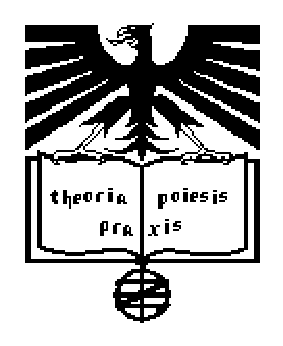
\includegraphics[height=60mm]{uaLogoOld}}} % the \FIG{} is optional
         {\ThesisYear}
  \TITLE{Bruno Manuel \newline de Moura Ramos}
        {Sistema de Recolha e Armazenamento Remoto de Informação Sensorial de um Processo Industrial usando Bases de Dados Múltiplas}
\EndTitlePage
\titlepage\ \endtitlepage % empty page


\TitlePage
  \vspace*{55mm}
  \TEXT{\textbf{o juri/the jury\newline}}
       {}
  \TEXT{presidente/president}
       {\textbf{ABC}\newline {\small
        Professor Catedratico da Universidade de Aveiro (por delegacao da Reitora da
        Universidade de Aveiro)}}
  \vspace*{5mm}
  \TEXT{vogais/examiners committee}
       {\textbf{DEF}\newline {\small
        Professor Catedratico da Universidade de Aveiro (orientador)}}
  \vspace*{5mm}
  \TEXT{}
       {\textbf{GHI}\newline {\small
        Professor associado da Universidade J (co-orientador)}}
  \vspace*{5mm}
  \TEXT{}
       {\textbf{KLM}\newline {\small
        Professor Catedratico da Universidade N}}
\EndTitlePage
\titlepage\ \endtitlepage % empty page

\TitlePage
  \vspace*{55mm}
  \TEXT{\textbf{agradecimentos~/\newline acknowledgements}}
       {Um obrigado aos que me ajudaram. (Adicionar agradecimentos)}
  \TEXT{}
       {}
\EndTitlePage
\titlepage\ \endtitlepage % empty page

\TitlePage
  \vspace*{55mm}
  \TEXT{\textbf{Palavras-chave}}
       {Base de dados relacional; rede de bases de dados; monitorização; monitorização remota; aplicação; \textit{web}.}
  \TEXT{Resumo}
       {Moldes de injeção têm uma vasta aplicabilidade no mundo industrial. Afim de melhorar a qualidade do produto final e reduzir falhas surgiu a necessidade de instrumentar e monitorizar moldes remotamente. Neste projeto desenvolveu-se uma rede de bases de dados relacionais e uma aplicação em ambiente \textit{Web}. A primeira garante uma transferência de valores segura e permanente de forma a criar um histórico. A segunda permite ao utilizador interagir com as bases de dados desenvolvidas podendo edita-las e consulta-las de forma a gerar relatórios.\\
       	No desenvolvimento deste projeto utilizou-se \textit{MySQL} e \textit{C} para criar e definir a rede de bases de dados resultando numa solução simples e funcional a baixo nível. Utilizou-se \textit{Apache}, \textit{PHP}, e \textit{HTML} para desenvolver e implementar a aplicação de forma a que esta seja multiplataforma e garanta um acesso remoto ao utilizador.\\
       	A solução proposta cumpre todos os objetivos definidos podendo ser já utilizada numa fase experimental apesar de necessitar alguns melhoramentos a nível de desempenho.}
\EndTitlePage
\titlepage\ \endtitlepage % empty page

\TitlePage
  \vspace*{55mm}
  \TEXT{\textbf{Abstract}}
       {Nowadays, it is usual to evaluate a work \ldots}
\EndTitlePage
\titlepage\ \endtitlepage % empty page


%
% Tables of contents, of figures, ...
%

\pagenumbering{roman}
\tableofcontents

\cleardoublepage
\listoffigures

\cleardoublepage
\listoftables


% The chapters (usually written using the isolatin font encoding ...)

\cleardoublepage
\pagenumbering{arabic}
\chapter{Introdução}
arquivo e monitorização de moldes.
\newpage
em branco
\newpage
em branco

\cleardoublepage
\chapter{Estado de Arte}
\section{Moldes de injeção}
\begin{figure}[H]
	\begin{center}
		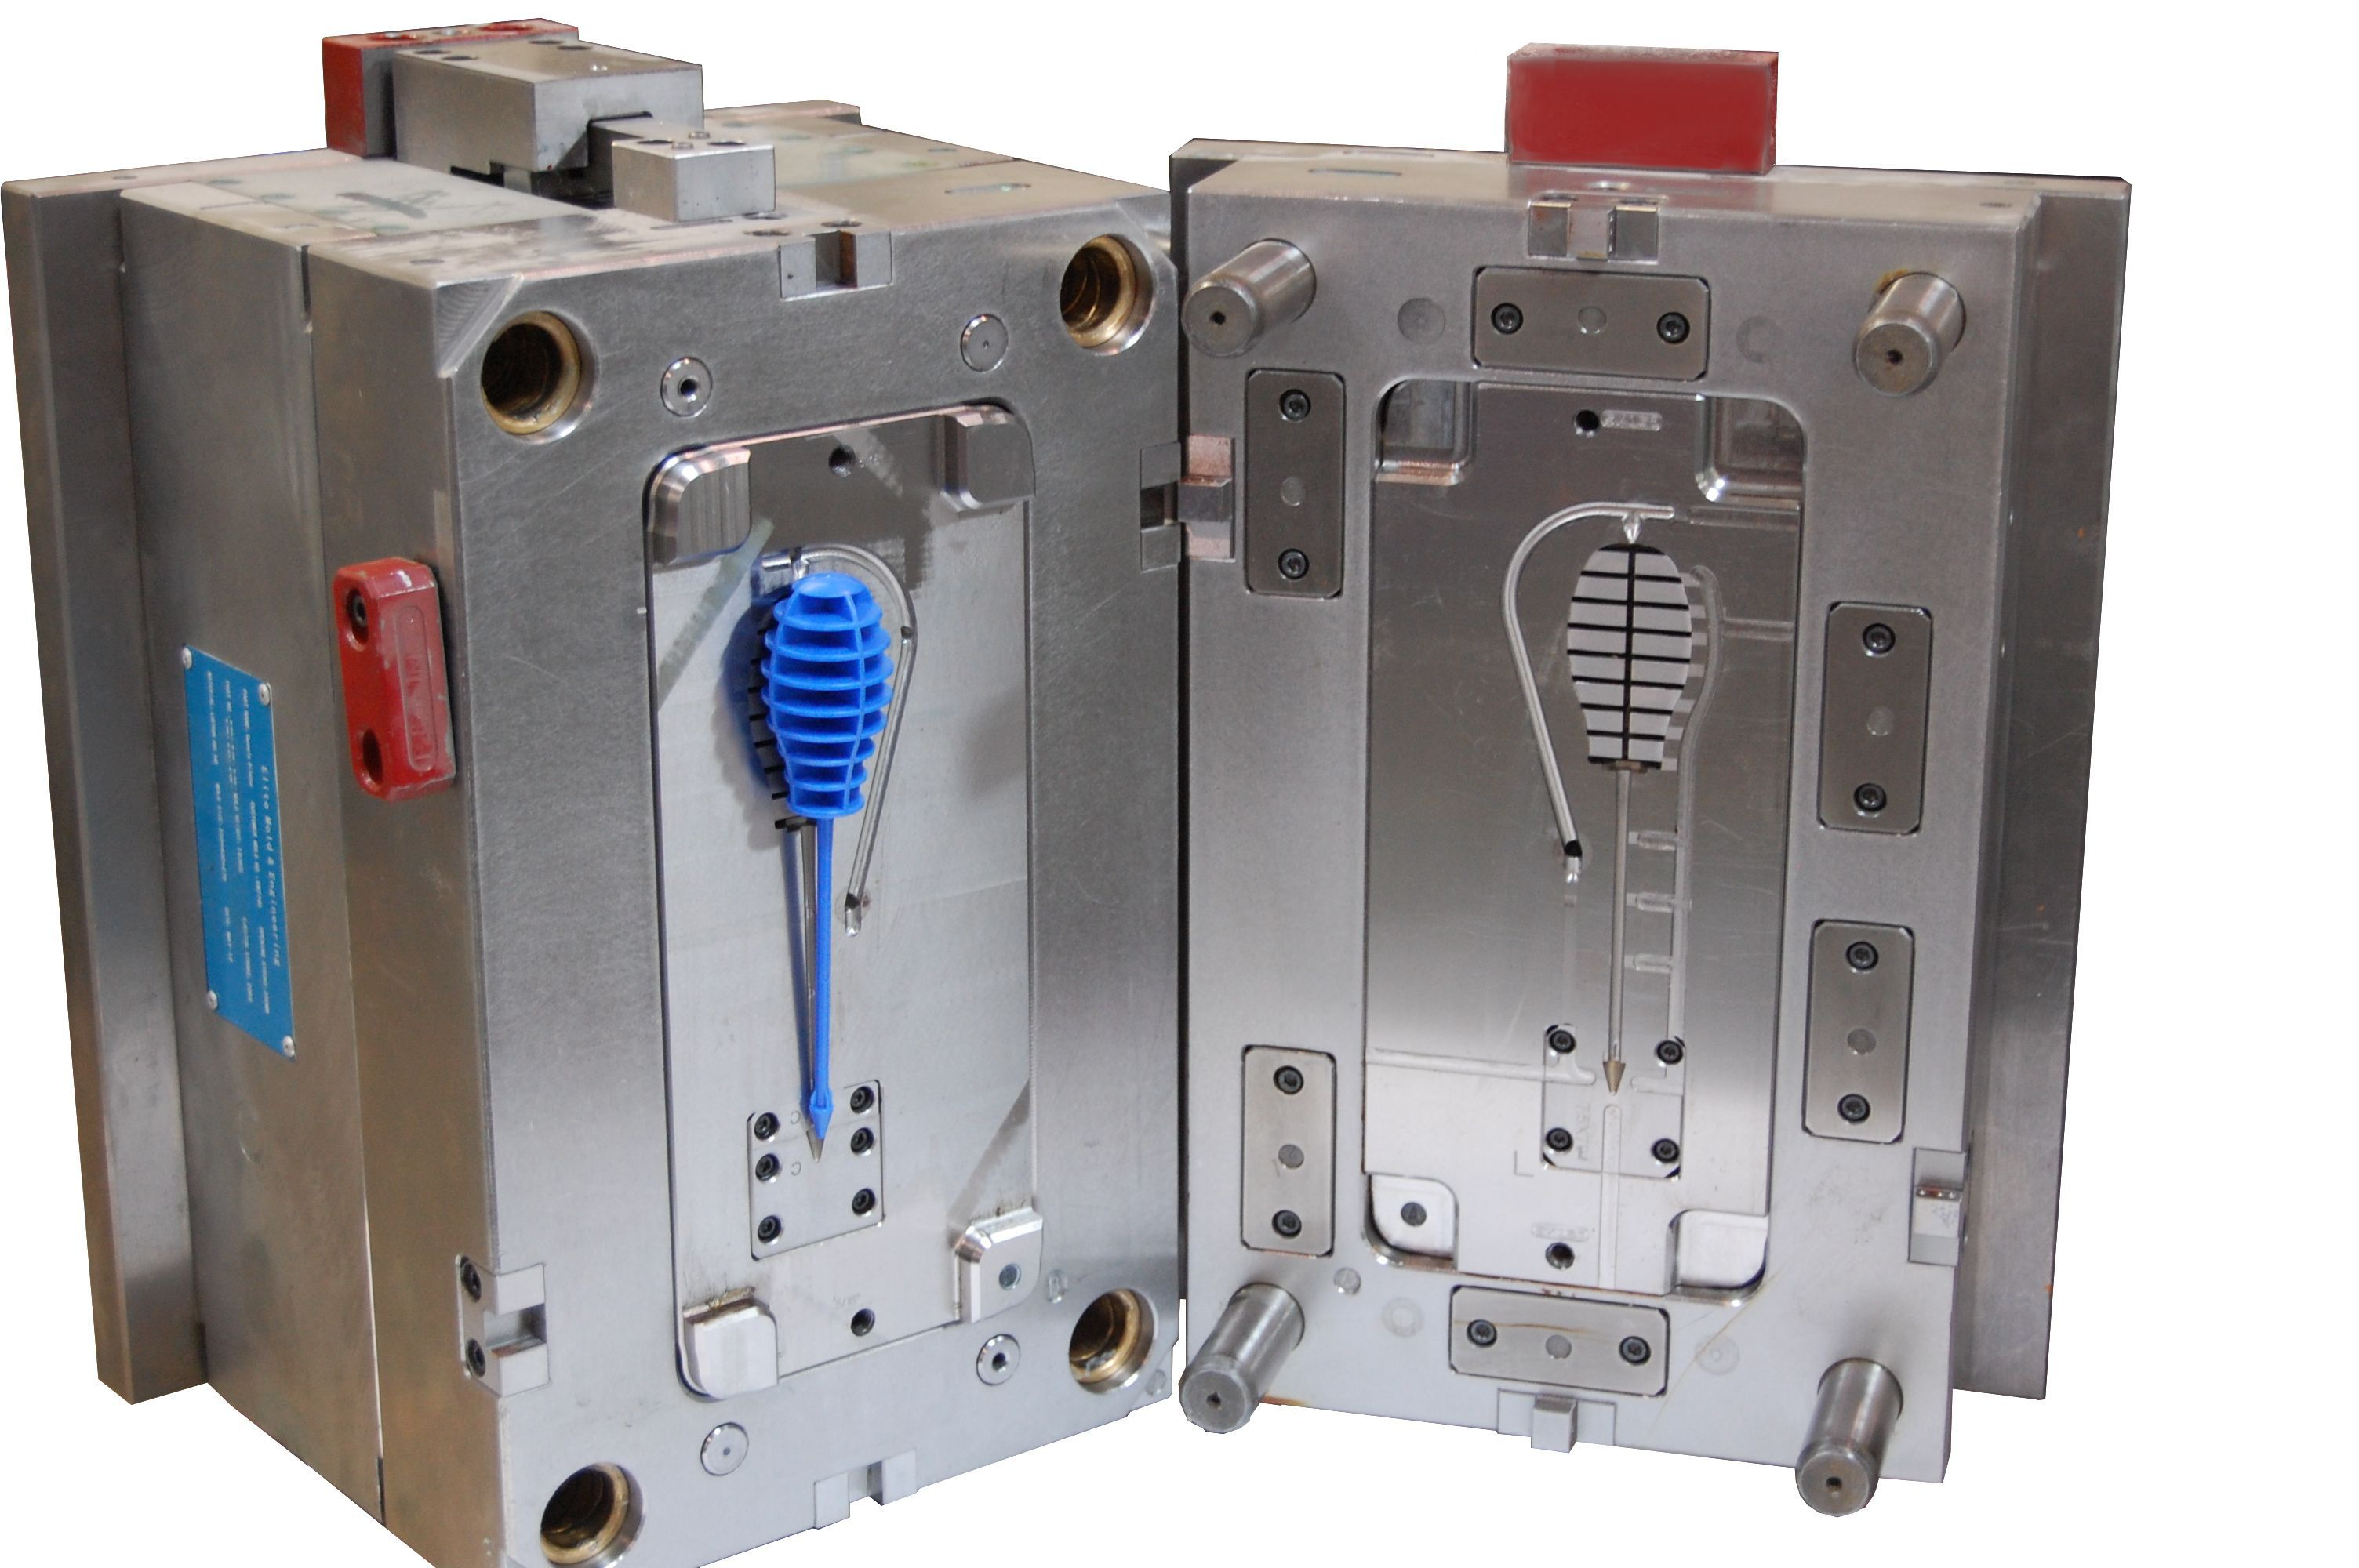
\includegraphics[width=0.9\textwidth]{molde} % Include the image placeholder.png
		\caption{Molde de injeção aberto com a peça realizada\cite{molde_imagem}}
		\label{fig:molde}
	\end{center}
\end{figure}
Moldagem é o processo mecânico de dar forma a um material no estado líquido usando um molde\cite{definicao_moldagem,definicao_moldar}. Um molde é uma ferramenta sólida oca desenvolvida para efeitos de fundição\cite{definicao_molde}. Esta é enchida com um material em estado liquido ou em pó como plástico, metal, cerâmica ou vidro\cite{Williams1975,Trovant1998,JanneyMarkA.Knoxville1991,Yan2009}.\par
A moldagem por injeção é particularmente útil na produção em massa de peças de plástico com elevada complexidade geométrica\cite{Shen,Shelesh}. Estas podem ser encontradas em todas as áreas da industria como por exemplo empacotamento, aviação, construção e eletrónica\cite{Ozcelik}. Neste processo, plástico quente é forçado para dentro de um molde frio com a forma desejada. O material cobre todas as feições do molde e vai endurecendo sobre o efeito de altas pressões. O processo de injeção pode ser divido em fases distintas\cite{Shen}:
\begin{itemize}[noitemsep]
	\item Fecho do molde
	\item Enchimento
	\item Compactação
	\item Abertura do molde
	\item Extração
\end{itemize}
Em 1868, John Wesley Hyatt inventou uma maneira de fazer bolas de bilhar injetando celuloide para dentro de um molde\cite{historia,patente1868}.\par
Em 1872 Jonh e o seu irmão Isaiah patentearam a primeira máquina de moldes de injeção. Esta era relativamente simples comparada às que são usadas hoje em dia na indústria. Consistia de um pequeno embolo para injetar plástico num molde através de um cilindro quente\cite{historia,patente1872}.\par
A indústria cresceu lentamente produzindo artigos de plástico como botões e pentes. Nos anos 40 a utilização de moldes de injeção cresceu por causa da Segunda Guerra Mundial que tinha uma grande procura de produtos baratos e produzidos em massa\cite{historia}.\par
Em 1946, James Hendry construiu a primeira máquina de moldes de injeção com um sem fim, revolucionando a indústria dos plásticos com um design para substituir o embolo de Hyatt. Este sem fim é colocado dentro do cilindro e mistura o material a ser moldado antes de ser injetado no molde. Isto permitiu que cor ou plástico reciclado fossem adicionados à mistura\cite{historia,patente1946}.\par
A qualidade de fabrico dos moldes e das peças produzidas evoluiu com o passar do tempo. A industria investiu em técnicas sofisticadas no desenvolvimento de moldes, para que estes não contenham falhas, e no uso de materiais com qualidade elevada para evitar o desgaste da ferramenta. No entanto, dificilmente se atinge peças com a qualidade desejada unicamente através das ferramentas desenvolvidas. É necessário implementar também técnicas de monitorização de qualidade\cite{Woll}.


\section{Base de dados relacional}
Bases de dados e sistemas de gestão de bases de dados são uma componente essencial na vida da sociedade moderna: muitos de nós realizamos ações todos os dias que envolvem interações com bases de dados. Por exemplo, o ato de depositar e levantar dinheiro num banco, reservar estadias e voos ou comprar alguma coisa online podem envolver alguém ou um algum programa informático que acede a uma base de dados\cite{Elmasri:2010:FDS:1855347}.\par
Esta tecnologia tem um impacto cada vez maior no uso dos computadores. É seguro afirmar que as bases de dados desempenham um papel crítico em quase todas as áreas onde são usados computadores\cite{Elmasri:2010:FDS:1855347}.\par
Uma base de dados é uma coleção organizada de dados que estão relacionados e que podem ser partilhados por múltiplas aplicações\cite{definicao_base_dados}. São considerados dados factos reais que podem ser registados e têm um significado implícito, como por exemplo, nomes, moradas e números de telefone. Uma base de dados tem uma fonte de onde os dados são provenientes, algum grau de interação com eventos do mundo real e uma audiência que está ativamente interessada no seu conteúdo\cite{Elmasri:2010:FDS:1855347}.\par
A implementação destas é garantida por parte de um sistema de gestão de base de dados. Este é um \textit{software} de que facilita os processos de definir, construir, manipular e partilhar bases de dados entre vários utilizadores e aplicações. Definir uma base de dados envolve especificar o tipo de dados, estruturas e restrições dos dados a serem armazenados. Construir é o processo de guardar dados e armazena-los num local definido pelo sistema de gestão de bases de dados. Manipular inclui funções como realizar \textit{queries} à base de dados e receber informação específica, altera-la de acordo com mudanças nas variáveis e gerar relatórios a partir dos dados presentes. Partilhar permite que múltiplos utilizadores e programas acedam à base de dados simultaneamente\cite{Elmasri:2010:FDS:1855347}.\par
Outras funções importantes fornecidas pelos sistemas de gestão de bases de dados incluem proteger e manter a base de dados durante um longo período de tempo. Proteger inclui proteção contra falhas de \textit{hardware} e \textit{software} e segurança contra acessos maliciosos ou não autorizados. Tipicamente uma grande base de dados pode ter um tempo de vida de vários anos, então o sistema de gestão de bases de dados tem de fornecer ferramentas para manter a base de dados de forma a permitir que o sistema evolua com novos requerimentos que surjam ao longo do tempo\cite{Elmasri:2010:FDS:1855347}.
Para completar estas definições iniciais, chama-mos sistema de base de dados ao conjunto das bases de dados com o sistema de gestão de bases de dados como representado na \autoref{fig:relacional1}.
\begin{figure}[H]
	\begin{center}
		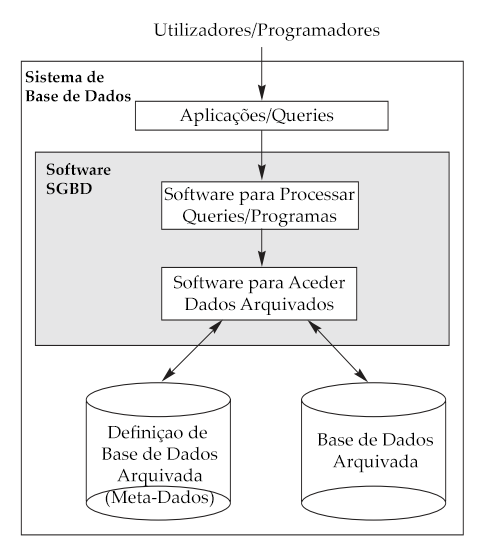
\includegraphics[width=0.7\textwidth]{SGBD} % Include the image placeholder.png
		\caption{Esquema simplificado de um sistema de bases de dados}
		\label{fig:relacional1}
	\end{center}
\end{figure}
O modelo relacional foi primeiramente introduzido por Ted Codd do \textit{IBM Research} em 1970\cite{Elmasri:2010:FDS:1855347,Codd} e atraiu imediatamente atenção pela sua simplicidade e base matemática. O modelo utiliza o conceito matemático de $ " $relação$ " $ representado por tabelas e é baseado na teoria dos conjuntos\cite{Elmasri:2010:FDS:1855347}.\par
As primeiras implementações comerciais do modelo relacional ficaram disponíveis no inicio dos anos 80, como o \textit{SQL/DS} no sistema operativo \textit{MVS} do \textit{IBM} e o sistema de gestão de base de dados \textit{Oracle}. Desde aí, o modelo tem sido implementado num grande número de sistemas comerciais. Os sistemas de gestão de bases de dados relacionais populares atualmente incluem \textit{DB2} e \textit{Informix Dynamic Server} (do \textit{IBM}), \textit{Oracle} e \textit{Rdb} (da \textit{Oracle}), \textit{Sybase} (da \textit{Sybase}) e \textit{SQLServer} e \textit{Access} (da \textit{Microsoft}). Existem também vários sistemas grátis como \textit{MySQL} e \textit{PostgreSQL}\cite{Elmasri:2010:FDS:1855347}.\par
Modelos de dados que procederam o relacional incluem os modelos hierárquicos e de rede. Estes foram propostos nos anos 60 e foram implementados nos primeiros sistemas de gestão de bases de dados nos anos 60 e 70. Estes modelos tiveram bastante importância na história das bases de dados e são referidos atualmente como sistemas de bases de dados \textit{legacy}\cite{Elmasri:2010:FDS:1855347}.

\subsection{Domínios, Atributos, Tuplos e Relações}
Um domínio é um conjunto atómico de valores. Atómico significa que cada valor num dado domínio é único e indivisível. Um método comum de especificar um domínio é especificar o tipo de dados do mesmo. Além disto, também é útil dar nomes aos domínios. Por exemplo, a informação de números de telemóvel pode ser guardada num domínio onde o seu tipo de dados é um inteiro de nove dígitos\cite{Elmasri:2010:FDS:1855347}.\par
Um esquema de relação é constituído por um nome de uma relação e uma lista de atributos. Cada atributo é o nome do papel desempenhado por domínio no esquema da relação. É possível múltiplos atributos terem o mesmo domínio\cite{Elmasri:2010:FDS:1855347}.\par 
A relação do esquema de relação é um grupo de múltiplos tuplos. Cada tuplo é um conjunto de valores ordenados que estão associados diretamente a um atributo.\par 
A \autoref{fig:relacional2} representa um exemplo do que foi dito anteriormente.
\begin{figure}[H]
	\begin{center}
		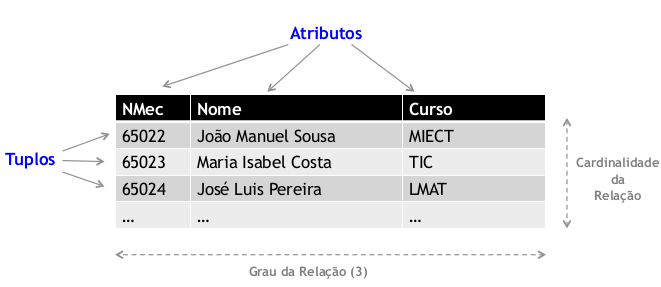
\includegraphics[width=0.9\textwidth]{exemplo_relacional} % Include the image placeholder.png
		\caption{Exemplo onde é possível observar a relação com os seus atributos e alguns tuplos}
		\label{fig:relacional2}
	\end{center}
\end{figure}

\subsection{Análise de requisitos}
A análise de requisitos é o primeiro passo necessário para definir uma base de dados. Este processo envolve uma comunicação com a entidade que deseja adquirir a base de dados e pode ser sumariza-do nos seguintes passos:
\begin{enumerate}
	\item Numa primeira fase realiza-se uma recolha detalhada de toda a informação referente ao problema do mundo real e retirar entidades, atributos, restrições, etc.
	\item Filtrar a informação de forma a remover redundâncias e informação pouco relevante
	\item Clarificar aspetos pouco claros
	\item Completar o problema com informação adicional necessária
	\item Distinguir dados de operações
\end{enumerate}
Este processo é transversal ao modelo de dados escolhido para realizar a base de dados. Para uma base de dados relacional é necessário identificar as chaves de uma relação:
\begin{itemize}
	\item Superchave - Conjunto de atributos que identificam de forma única dois tuplos distintos
	\item Chave candidata - são todas as superchaves que não podem ser mais simplificadas
	\item Chave primária - escolhida do conjunto de chaves candidatas e identifica de forma única o tuplo
	\item Chave única - restantes chaves candidatas que não foram escolhidas como chave primária
	\item Chave estrangeira - conjunto de atributos que é chave primária de outra relação
\end{itemize}
A escolha da chave primária pode ser feita de forma aleatória mas, priorizam-se chaves que identifiquem de forma natural um atributo. Por exemplo: uma pessoa pode ser identificada por um número de identificação, número de identificação fiscal ou pelo seu número de telefone dado que estes nunca se repetem. O número de identificação é mais natural para identificar uma pessoa do que o seu número de identificação fiscal e menos volátil do que o seu número de telefone, dado que este pode ser alterado.\par 
Para realizar um Diagrama Entidade Relação são necessárias informações sobre a relação entre as entidades, a cardinalidade e a obrigatoriedade de participação na relação. Estas são deduzidas durante a análise de requisitos mas serão explicadas na \autoref{subchap:DER}.

\subsection{Diagrama Entidade Relação}
\label{subchap:DER}
A representação lógica dos dados é uma componente importante na área das bases de dados. Existem vários modelos para esta representação antes da criação do modelo entidade-relação apresentado por P. P. Chen em 1976, sendo os mais conhecidos os modelos em rede, relacional e entidade. Estes modelos têm as suas vantagens e desvantagens. O modelo em rede permite uma vista mais natural dos dados dividindo-os em entidades e relações (até um determinado ponto), mas a sua capacidade de garantir independência dos dados foi superada. O modelo relacional consegue ter um grande grau de independência dos dados, mas pode perder alguma informação semântica importante sobre o mundo real. O modelo de entidade também consegue um grande grau de independência dos dados, mas a forma visualizar os dados não é tão fácil para algumas pessoas\cite{Chen}.\par
O modelo entidade-relação adota uma vista mais natural em que o mundo real consiste de entidades e relações, incorpora alguma informação semântica importante sobre o mundo real e consegue ter um grande grau de independência de dados. O modelo entidade-relação é baseado na teoria das relações e foi desenvolvido com o objetivo de servir de base para um sistema de visualização de dados unificado\cite{Chen}.\par
O diagrama entidade relação é uma representação gráfica da análise de requisitos realizada anteriormente baseada no modelo entidade-relação. Este diagrama não é determinístico pois, para uma mesma análise, podem nascer diferentes diagramas que cumprem todos os requisitos.\par
Um diagrama é constituído elementos como entidades, atributos e relações. Uma entidade é algo que existe no mundo real como uma pessoa ou um carro. Um atributo é uma característica da entidade como uma pessoa tem um nome e um carro tem uma matricula. Uma relação é como uma ou mais entidades interagem entre si como uma pessoa tem um carro\cite{Chen}.\par 
Passando à notação, as entidades são representadas por caixas retangulares, os atributos por caixas ovais e as relações por caixas em forma de losango como mostra a \autoref{fig:der1}. Os atributos sublinhados representam a chave primária da entidade.
\begin{figure}[H]
	\begin{center}
		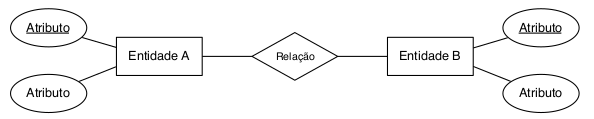
\includegraphics[width=1\textwidth]{notacao1} % Include the image placeholder.png
		\caption{Representação de entidades, relações e atributos}
		\label{fig:der1}
	\end{center}
\end{figure}
As entidades e relações podem ser fortes e fracas. Uma entidade forte não depende de outras entidades, enquanto uma entidade fraca necessita de ser identificada em conjunto com uma entidade forte. As relações fortes definem a ou as entidades fortes que identificam uma entidade fraca entre as quais esta se relaciona. As entidades fracas são representadas por caixas retangulares com linha dupla e as relações fortes são identificadas por um losango de linha dupla como representado na \autoref{fig:der2}.
\begin{figure}[H]
	\begin{center}
		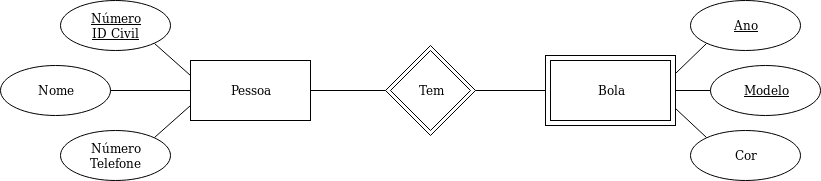
\includegraphics[width=0.8\textwidth]{notacao2} % Include the image placeholder.png
		\caption{Representação de entidades e relações fortes e fracas}
		\label{fig:der2}
	\end{center}
\end{figure}
\newpage
Para completar a relação entre entidades é necessário identificar também o grau, cardinalidade e obrigatoriedade de participação de uma relação. Quanto ao grau uma relação pode ser unária, binária ou ternária como representado na \autoref{fig:der3}. As relações ternárias podem ser decompostas em relações binárias. %como mostra a \autoref{fig:der4}.
\begin{figure}[H]
	\begin{center}
		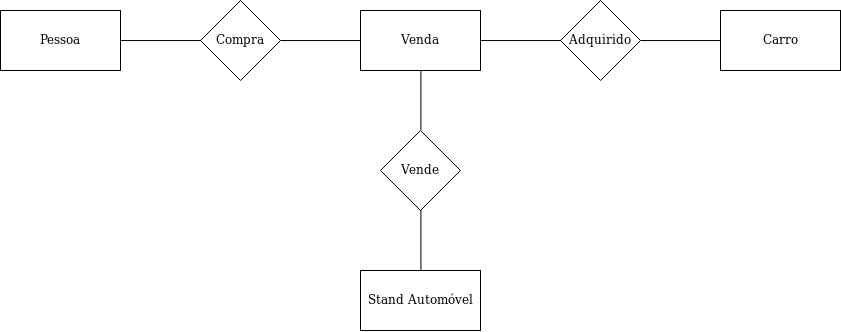
\includegraphics[width=0.7\textwidth]{notacao6} % Include the image placeholder.png
		\caption{Representação dos vários graus das relações (NECESSITA EDIÇÃO)}
		\label{fig:der3}
	\end{center}
\end{figure}
%\begin{figure}[H]
%	\begin{center}
%		
\includegraphics[width=0.7\textwidth]{placeholder} % Include the image placeholder.png
%		\caption{exemplo}
%		\label{fig:der4}
%	\end{center}
%\end{figure}
As relações podem também ser múltiplas, ou seja, mais do que uma relação entre entidades como demonstrado na \autoref{fig:der8}.
\begin{figure}[H]
	\begin{center}
		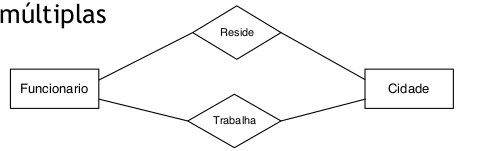
\includegraphics[width=0.7\textwidth]{notacao3} % Include the image placeholder.png
		\caption{Representação de múltiplas relações entre duas entidades}
		\label{fig:der8}
	\end{center}
\end{figure}
Quanto à cardinalidade uma relação pode ser de três tipos:
\begin{itemize}[noitemsep]
	\item 1 para 1
	\item N para 1
	\item N para M
\end{itemize}
A \autoref{fig:der5} apresenta uma representação visual destas cardinalidades e a \autopageref{fig:der6} apresenta a notação da cardinalidade definida por Chen.
\begin{figure}[H]
	\begin{center}
		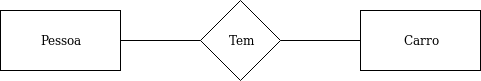
\includegraphics[width=0.7\textwidth]{notacao4} % Include the image placeholder.png
		\caption{Diagrama dos vários tipos de cardinalidade}
		\label{fig:der5}
	\end{center}
\end{figure}
\begin{figure}[H]
	\begin{center}
		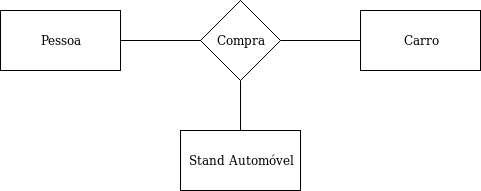
\includegraphics[width=0.7\textwidth]{notacao5} % Include the image placeholder.png
		\caption{Notação da cardinalidade de Chen}
		\label{fig:der6}
	\end{center}
\end{figure}
A obrigatoriedade de participação numa relação define se uma entidade tem de participar obrigatoriamente numa relação. Esta é representada por uma linha dupla na conexão com a relação como representado na Figura \ref{fig:der9}. %e \ref{fig:der10}. 
\begin{figure}[H]
	\begin{center}
		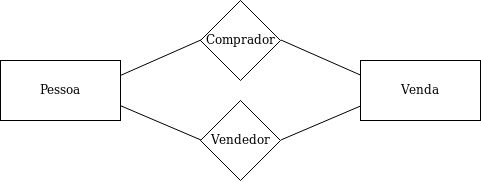
\includegraphics[width=0.7\textwidth]{notacao7} % Include the image placeholder.png
		\caption{Representação da obrigatoriedade de participação}
		\label{fig:der9}
	\end{center}
\end{figure}
%\begin{figure}[H]
%	\begin{center}
%		
\includegraphics[width=0.7\textwidth]{placeholder} % Include the image placeholder.png
%		\caption{exemplo}
%		\label{fig:der10}
%	\end{center}
%\end{figure}
Os atributos também podem ser de tipos diferentes. Estes podem ser derivados, compostos ou multi-valor como mostra a \autoref{fig:der11}
\begin{figure}[H]
	\begin{center}
		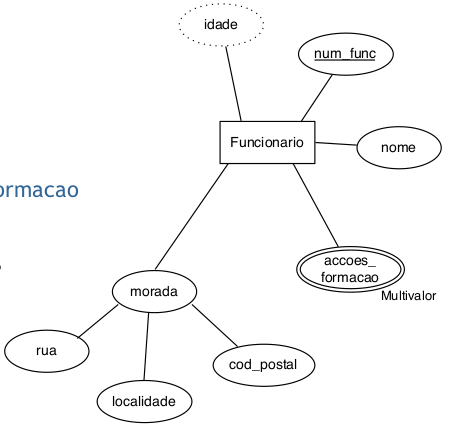
\includegraphics[width=0.7\textwidth]{notacao8} % Include the image placeholder.png
		\caption{Representação dos vários tipos de atributos. Os atributos derivados são representados a tracejado, os compostos têm sub-atributos associados a si e os multi-valor são representados com linha dupla}
		\label{fig:der11}
	\end{center}
\end{figure}

\subsection{Esquema Relacional}
O esquema relacional incluí todas as relações que concretizam uma base de dados. Cada relação é representada pelos seus atributos, tendo os atributos chave sublinhados. Quando atributos de relações diferentes representam o mesmo elemento do mundo real, estes são conectados. Quando um elemento aparece em relações diferentes significa que numa destas, o elemento, é atributo chave da relação e assim sendo, os restantes atributos são considerados chaves estrangeiras. São representados com a ligação ao atributo que serve de chave primária como demonstrado na \autoref{fig:er1}\cite{Chen}.
\begin{figure}[H]
	\begin{center}
		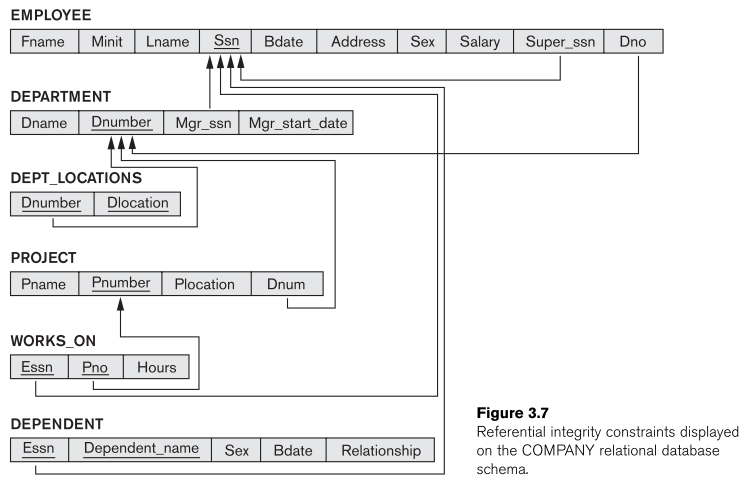
\includegraphics[width=0.7\textwidth]{notacao9} % Include the image placeholder.png
		\caption{Representação de um esquema relacional com as ligações das chaves estrangeiras}
		\label{fig:er1}
	\end{center}
\end{figure}
Este esquema pode ser deduzido a partir do diagrama entidade relação onde as entidades se traduzem em relações e as relações do diagrama representam as chaves estrangeiras no esquema relacional.

\section{\textit{Structured Query Language}}
A linguagem \textit{SQL} é considerada uma das maiores razões para o sucesso comercial das bases de dados relacionais. Porque se tornou normal a sua utilização em bases de dados relacionais, os utilizadores tiveram menos preocupações a transferir as suas aplicações de outros tipos de bases de dados - por exemplo, bases de dados hierárquicas e em rede - para uma base de dados relacional. Isto porque se um sistema de gestão de bases de dados não cumprisse os requisitos definidos, não era problemático transferir a solução para outro sistema de gestão de bases de dados dado que ambos utilizam a mesma linguagem. Na realidade existem várias sub-versões desta linguagem dependentes de cada sistema de gestão de bases de dados. No entanto, se o utilizador se limitar apenas às funções standard desta linguagem a mudança de sistema é bastante simplificada. Outra vantagem de ter uma linguagem normalizada é que uma aplicação pode utilizar informação de bases de dados em sistemas de gestão de bases de dados diferentes ao mesmo tempo\cite{Elmasri:2010:FDS:1855347}.\par 
O nome \textit{SQL} atualmente significa \textit{Structured Query Language}. Originalmente era chamado \textit{SQUEL} de \textit{Structured English QUEry Language}, foi desenhado e implementado no \textit{IBM Research} como uma interface experimental para o sistema de bases de dados relacionais \textit{SYSTEM R. SQL}. Um esforço conjunto entre o \textit{American National Standards Institute} (\textit{ANSI}) e a \textit{International Standards Organization} (\textit{ISO}) conduziu à normalização da versão do \textit{SQL} chamado SQL-86 ou SQL1. Surgiu depois uma versão expandida chamada SQL-92 ou SQL2. A seguinte versão reconhecida é o SQL:1999 ou SQL3. Dois \textit{updates} de depois resultaram nas versões SQL:2003 e SQL:2006\cite{Elmasri:2010:FDS:1855347}. Sendo a atualização mais recente em 2016.\par 
O \textit{SQL} é uma linguagem básica para realizar \textit{queries} dividida em dois campos principais, \textit{DDL} e \textit{DML}. \textit{DDL} ou \textit{Data Definition Language} são as \textit{queries} que permitem definir e construir uma base de dados. \textit{DML} ou \textit{Data Manipulation Language} são as \textit{queries} que permitem interagir com os dados\cite{Elmasri:2010:FDS:1855347}. Estas serão mais exploradas na \autoref{subchap:mysql}.

%\section{Tecnologias existentes}

\section{\textit{Software} utilizado}
Para desenvolver as redes de bases de dados e aplicação escolheram-se os \textit{softwares} e linguagens apresentados neste capítulo. Como a solução será futuramente implementada em ambiente empresarial, definiu-se que não se deve usar \textit{softwares} que estejam em versão \textit{beta}. Além disto sugere-se que sejam também gratuitos.

\subsection{\textit{Ubuntu}}
\begin{figure}[H]
	\begin{center}
		
\includegraphics[width=0.3\textwidth]{ubuntu} % Include the image placeholder.png
		\caption{Logótipo do \textit{Ubuntu}}
		\label{fig:linux}
	\end{center}
\end{figure}
Escolheu-se o \textit{Ubuntu} 16.04LTS como sistema operativo para os sistemas usados neste projeto, representado na \autopageref{fig:linux}. Este é uma distribuição do \textit{Linux} baseado no \textit{Debian}. É um sistema operativo grátis e \textit{open source} desenvolvido pela \textit{Canonical}. A liberdade deste sistema operativo na área da programação criou uma comunidade de utilizadores que ajudam a pesquisar e desenvolver este sistema operativo.\cite{ubuntu}.\par 
A \textit{Canonical} encarrega-se de garantir \textit{updates} de segurança e performance de forma regular. Apesar de não ser infalível o \textit{Linux} é um dos sistemas mais estáveis e menos provável de ser afetado por vírus, dado que a maior parte destes são desenhados para afetar sistemas operativos mais populares como o \textit{Windows}.

\subsection{\textit{MySQL}}
\label{subchap:mysql}
\begin{figure}[H]
	\begin{center}
		
\includegraphics[width=0.5\textwidth]{mysql} % Include the image placeholder.png
		\caption{Logótipo do \textit{MySQL}}
		\label{fig:mysql}
	\end{center}
\end{figure}
Escolheu-se o \textit{MySQL}, representado na \autoref{fig:mysql}, como sistema de gestão de bases de dados relacionais para construir e utilizar as bases de dados usadas neste projeto, dada a sua simplicidade e velocidade de resposta. Existem outras ofertas gratuitas como o \textit{SQLite} e o \textit{PostgreSQL}. O \textit{SQLite} funciona apenas localmente e não permite uma conexão remota que se procura como solução para o problema. O \textit{PostgreSQL} é um sistema robusto que permite realizar tarefas que o \textit{MySQL} não consegue realizar. No entanto, dada a simplicidade da base de dados prevista na fase de projeto, não é necessário usar uma ferramenta tão completa e robusta\cite{mysqlvs}.\par 
O \textit{MySQL} é o mais popular e o sistema de gestão de bases de dados relacionais e o mais usado\cite{mysqlvs}. Garante um acesso múltiplo, rápido e robusto a uma base de dados no servidor. Foi desenvolvido para lidar com grandes quantidades de informação e \textit{softwares} com utilização massiva\cite{mysql}.\par 
O \textit{MySQL} oferece soluções gratuitas e pagas, \textit{Community} e \textit{Enterprise}, respetivamente. A primeira recebe menos \textit{updates} e correções que a solução paga. Tem também algumas funcionalidades bloqueadas e um limite na capacidade de sensivelmente 4Gb\cite{mysql}. Estas limitações não afetam o projeto e como tal opta-se pela solução gratuita deste \textit{software}.\par
Como referido anteriormente os vários sistemas de gestão de bases de dados possuem as suas próprias sub-versões da linguagem \textit{SQL} e, o \textit{MySQL}, não é exceção. Existem vários comandos presentes nas componentes \textit{DDL} e \textit{DML} desta linguagem, a seguinte lista enumera os comandos principais utilizados neste projeto:
\begin{itemize}
	\item \textbf{SHOW DATABASES/TABLES} - mostra todas as bases de dados ou tabelas da base de dados (\textit{MySQL})
	\item \textbf{CREATE DATABASE/TABLE} - criar bases de dados ou tabelas
	\item \textbf{DROP DATABASE/TABLE} - eliminar bases de dados ou tabelas
	\item \textbf{SELECT FROM} - visualizar tuplos de uma tabela
	\item \textbf{INSERT} - inserir tuplos numa tabela
	\begin{itemize}
		\item \textbf{INTO} - se forem inseridos múltiplos tuplos e um não respeitar as restrições de integridade definidas, nenhum tuplo é inserido
		\item \textbf{IGNORE} - se forem inseridos múltiplos tuplos e um não respeitar as restrições de integridade, esse é descartado e os restantes são inseridos na tabela (\textit{MySQL})
	\end{itemize}
	\item \textbf{DELETE} - elimina tuplos de uma tabela
	\item \textbf{UPDATE} - altera tuplos de uma tabela
	\item \textbf{GRANT} - dar privilégios a um utilizador
\end{itemize}
A \textit{querie} do tipo SELECT permite adicionar condições do tipo:
\begin{itemize}
	\item \textbf{WHERE} - definir parâmetros de busca de um atributo
	\item \textbf{GROUP BY} - permite agrupar informação permitindo operações matemáticas sobre valores, por exemplo: contagem, soma, média, etc.
	\item \textbf{ORDER BY} - escolher a ordem dos tuplos
\end{itemize}
As \textit{queries} do tipo DELETE e UPDATE  também permitem utilizar a condição WHERE.\par 
Na criação das tabelas atribuem-se o nome dos atributos e o seu respetivo domínio. O \textit{MySQL} oferece vários tipos de dados, dos quais foram usados:
\begin{itemize}
	\item \textbf{VARCHAR(n)} - \textit{string} com tamanho máximo n
	\item \textbf{INT} - inteiro entre -2147483648 e +2147483647
	\item \textbf{TINYINT} - inteiro entre -128 e +127
	\item \textbf{FLOAT} - numérico com casa decimais
	\item \textbf{DATETIME} - data e hora no formato AAAA-MM-DD HH:MM:SS
\end{itemize}
Define-se também as restrições de integridade:
\begin{itemize}
	\item \textbf{PRIMARY KEY} - define chave primária
	\item \textbf{UNIQUE} - define chave única
	\item \textbf{FOREIGN KEY REFERENCES} - define a chave estrangeira e o atributo de referência
\end{itemize}
Estas restrições ou \textbf{CONSTRAINTS} podem e devem ser atribuídas um nome de forma a identifica-las em mensagens de erro. Além disto é possível definir o comportamento de uma restrição de uma chave estrangeira quando o atributo de referencia é alterado (\textbf{ON UPDATE}) ou eliminado (\textbf{ON DELETE}):
\begin{itemize}
	\item \textbf{NO ACTION} - não deixa realizar a ação
	\item \textbf{CASCADE} - todas as chaves estrangeiras dependentes do atributo de referencia são alteradas ou eliminadas de acordo com este
	\item \textbf{SET NULL} - altera o valor da chave estrangeira para NULL
	\item \textbf{SET DEFAULT} - altera o valor da chave estrangeira para um valor predefinido
\end{itemize}
O valor NULL representa um valor de um atributo que não existe ou é desconhecido, adiciona-se \textbf{NOT NULL} a um atributo quando este não pode assumir este valor.\par 
Estes são os comandos e conceitos principais que surgem ao longo deste documento. Como referido anteriormente e é possível observar aqui, o \textit{SQL} é uma linguagem simples e auto-explicativa.

\subsection{\textit{C}}
\begin{figure}[H]
	\begin{center}
		
\includegraphics[width=0.4\textwidth]{gcc} % Include the image placeholder.png
		\caption{Logótipo do \textit{GNU}}
		\label{fig:gcc}
	\end{center}
\end{figure}
Escolheu-se utilizar \textit{C} no desenvolvimento deste projeto devido à afinidade com esta linguagem e com o facto do \textit{MySQL} disponibilizar protocolos oficiais e documentação de comunicação com esta linguagem\cite{mysql}.\par
O \textit{C} é uma linguagem para todos os tipos de problemas e importante no mundo da programação. Originalmente desenvolvido por Dennis Ritchie entre 1969 e 1973 no \textit{Bell Labs} e usado para re-implementar o sistema operativo \textit{Unix}. Desde então esta tornou-se uma das linguagens de programação mais popular de sempre com uma oferta de vários compiladores existentes no mercado. O \textit{C} foi então normalizado pelo \textit{ANSI} em 1989 e consequentemente pelo \textit{ISO}.\par 
No projeto usa-se o \textit{GNU Compiler Collection} (\textit{GCC}), representado na \autoref{fig:gcc}, como compilador dos programas em \textit{C}. Este foi desenvolvido primeiramente para o sistema operativo \textit{GNU} e focou-se em ser gratuito e garantir liberdade de programação ao utilizador. Conta com uma comunidade ativa que desenvolvem constantemente novas soluções e \textit{updates} regulares ao compilador de forma a que este não fique desatualizado\cite{gcc}.

\subsection{\textit{Apache}}
\begin{figure}[H]
	\begin{center}
		
\includegraphics[width=0.6\textwidth]{apache} % Include the image placeholder.png
		\caption{Logótipo do \textit{Apache}}
		\label{fig:apache}
	\end{center}
\end{figure}
Escolheu-se utilizar \textit{Apache HTTP Server}, representado na \autoref{fig:apache} como servidor \textit{HTTP} para a aplicação \textit{Web}. Este foca-se em ser um servidor gratuito e garantir uma solução segura, eficiente e extensível\cite{apache}.\par
Lançado em 1995, tornou-se no \textit{software} mais utilizado pelas empresas para correr os seus \textit{sites}. Atualmente na versão 2.4, realizam \textit{updates} constantes ao programa para o manter estável e atualizado\cite{apache}.

\subsection{\textit{HTML}, \textit{JS} e \textit{PHP}}
\begin{figure}[H]
	\begin{center}
		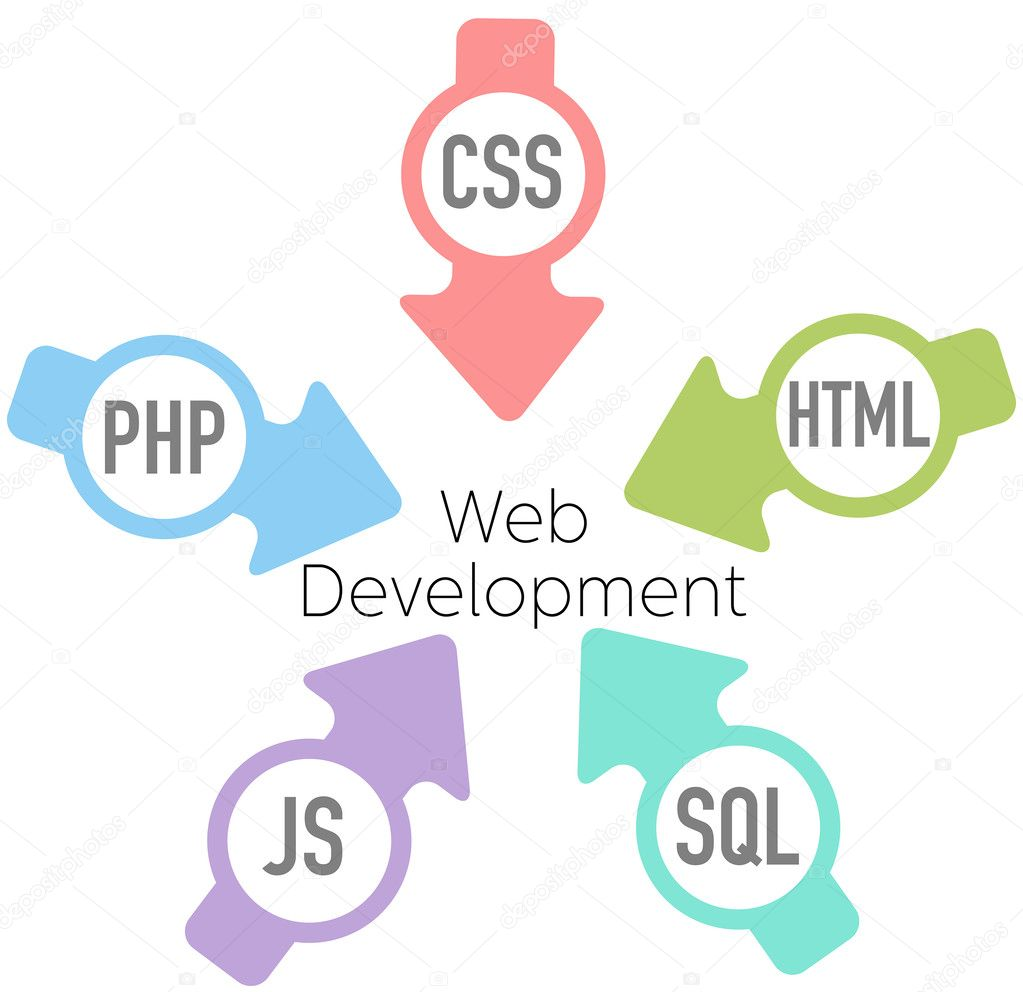
\includegraphics[width=0.5\textwidth]{web} % Include the image placeholder.png
		\caption{Representação da ferramenta mais usada para desenvolver aplicações em ambiente \textit{Web}}
		\label{fig:web}
	\end{center}
\end{figure}
Escolheu-se \textit{HTML}, \textit{JS} e \textit{PHP} para desenvolver a aplicação \textit{Web} deste projeto. Junto com \textit{SQL} e \textit{CSS} formam o conjunto de ferramentas mais usadas no desenvolvimento de aplicações \textit{Web} no mercado, representado na \autoref{fig:web}.\par 
\textit{HTML} ou \textit{Hyper Text Markup Language} descreve a estrutura da página \textit{Web} desenvolvida. Possuí elementos que funcionam como blocos para as páginas permitindo a criação de uma interface com um utilizador. \textit{CSS} ou \textit{Cascading Style Sheets} descreve como os elementos HTML devem ser dispostos na página, permitindo o desenvolvimento de uma interface mais apelativa. \textit{JS} ou \textit{JavaScript} permite interagir e alterar o código \textit{HTML} e \textit{CSS} criando uma interface mais interativa. Permite também desenvolver códigos e funções que são executadas no browser do cliente. \textit{PHP} ou \textit{PHP:Hypertext Preprocessor} permite desenvolver funções para aplicação que executam do lado do servidor. \textit{JS} e \textit{PHP} realizam ambos funções diferindo apenas no local onde são executadas. Sem contar com a interação com o \textit{HTML} e \textit{CSS}, o \textit{PHP} pode substituir o \textit{JS} como linguagem para criação de funções do sistema. No entanto, isto pode causar problemas de desempenho dado que o servidor terá de correr funções de todos os utilizadores. Assim sendo define-se que o uso do \textit{PHP} deve ser limitado a funções de sistema mais importantes, como conectar a uma base de dados em \textit{SQL}, e o \textit{JS} deve ser usado no desenvolvimento de funções de aplicação mais triviais.


\cleardoublepage
\chapter{Proposta de Solução}
\section{Infraestrutura de dados}
\newpage
em branco

\section{Base de Dados}
\subsection{Análise de Requisitos}
\newpage
em branco
\newpage
em branco

\newpage
em branco
\subsection{Desenho conceptual e esquema lógico}
\newpage
em branco

\newpage
em branco
\subsection{Construção da base de dados}
\begin{table}
	\caption{Domínio dos atributos}
\end{table}
\newpage
em branco

\newpage
em branco
\subsection{Programa de transferência}

\newpage
em branco
\subsection{Gestão de \textit{backups}}
\label{subchap:backups}
\newpage
em branco
\newpage
em branco

\newpage
em branco
\subsection{Simulador}

\subsection{Utilizadores}
\newpage
em branco

\cleardoublepage
\chapter{Aplicação}
Aplicação desenvolvida em ambiente  \textit{Web} com o objetivo de ser multiplataforma, permitir acesso remoto e sem recorrer a instalação de \textit{softwares} nos dispositivos dos utilizadores. Esta corre num servidor \textit{Apache} e foi desenvolvida com \textit{PHP} e \textit{HTML}. Este capítulo descreve a adaptação da infraestrutura desenvolvida e as várias funcionalidades da aplicação.

\section{Adaptação da infraestrutura}
Afim de garantir uma maior integridade dos dados inseridos pela aplicação, instala-se no servidor local uma nova base de dados temporária local. Aqui os utilizadores têm a liberdade para adicionar, alterar e apagar informação sem consequências no sistema antes destas serem introduzidas nas bases de dados central e local como representado na \autoref{fig:adap1}. Como referido anteriormente, esta base de dados difere das restantes, não contendo em si as tabelas fase e registos.
\begin{figure}[H]
	\begin{center}
		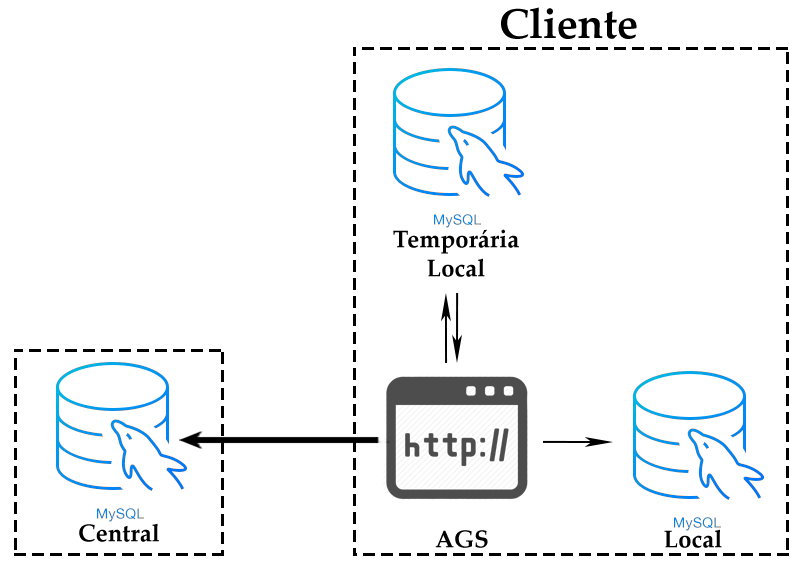
\includegraphics[width=0.65\textwidth]{Aplicacao_temp_local_central} % Include the image placeholder.png
		\caption{Esquema ligação Aplicação-bases de dados. A aplicação comunica com a base de dados temporária local e depois regista os valores desta nas bases de dados central e local}
		\label{fig:adap1}
	\end{center}
\end{figure}

\section{Interface gráfica}
A aplicação divide-se em cinco partes distintas:
\begin{itemize}[noitemsep]
	\item \textit{Main}
	\item \textit{Login}
	\item Consultas
	\item Administração
	\item Conexão Local
\end{itemize}
As páginas \textit{Main}, \textit{Login}, Consultas e parte das funcionalidades da Administração foram realizadas para uma utilização geral. As páginas Conexão Local e as restantes funcionalidades da Administração foram realizadas para uma utilização local. A primeira visa um uso a partir de qualquer dispositivo e acessível a qualquer momento e a segunda foca-se num acesso local com o objetivo de configurar e definir a informação no servidor local. Por outras palavras, para o utilizador usar as funcionalidades destas páginas tem de aceder à aplicação no sistema local que se situa no cliente.\\
Instalar um molde é culminar de um projeto de elevada responsabilidade, esta ideia junto com a criação da base de dados temporária local serve para melhorar a qualidade da informação introduzida no sistema e diminuir as falhas.\\

\newpage
\subsection{\textit{Main}}
\begin{figure}[H]
\centering
	\begin{minipage}{1.\textwidth}
		\begin{center}
			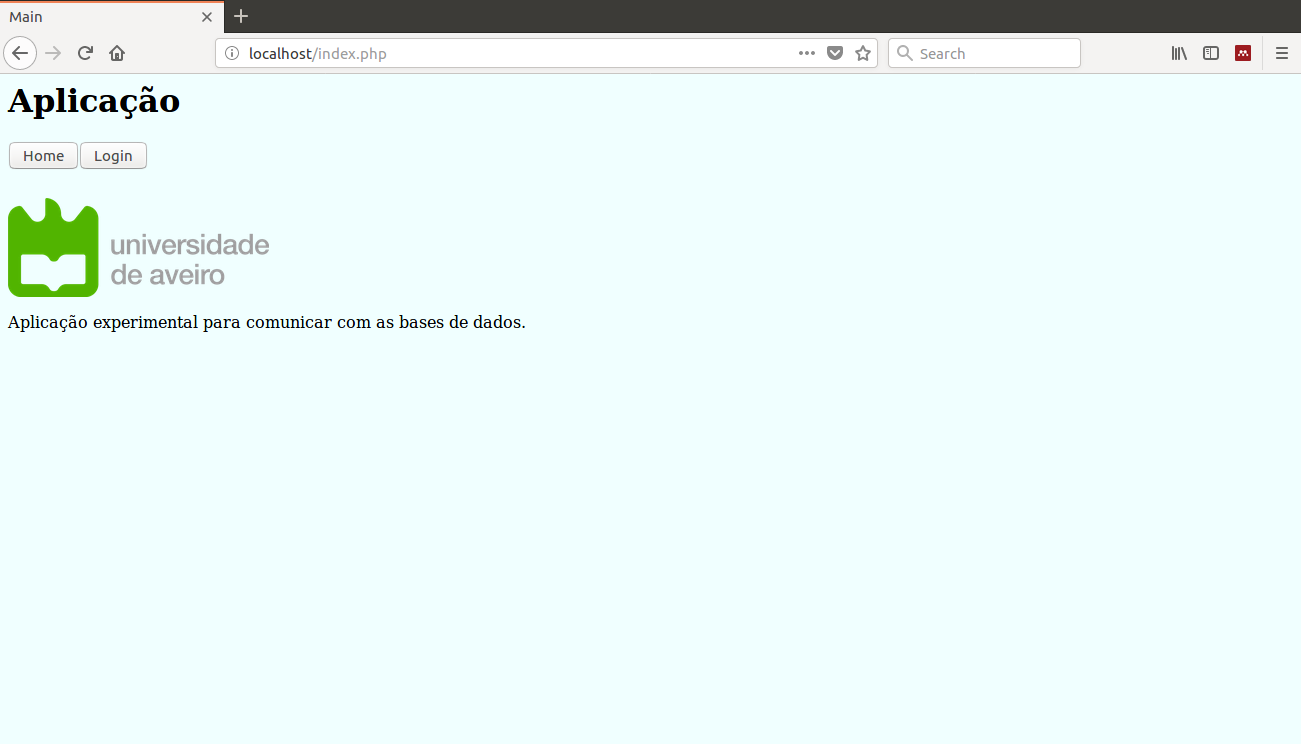
\includegraphics[width=0.85\textwidth]{main01} % Include the image placeholder.png
			\subcaption{Sem \textit{login}}
			\label{fig:main1}
		\end{center}
	\end{minipage}
	\begin{minipage}{1.\textwidth}
		\begin{center}
			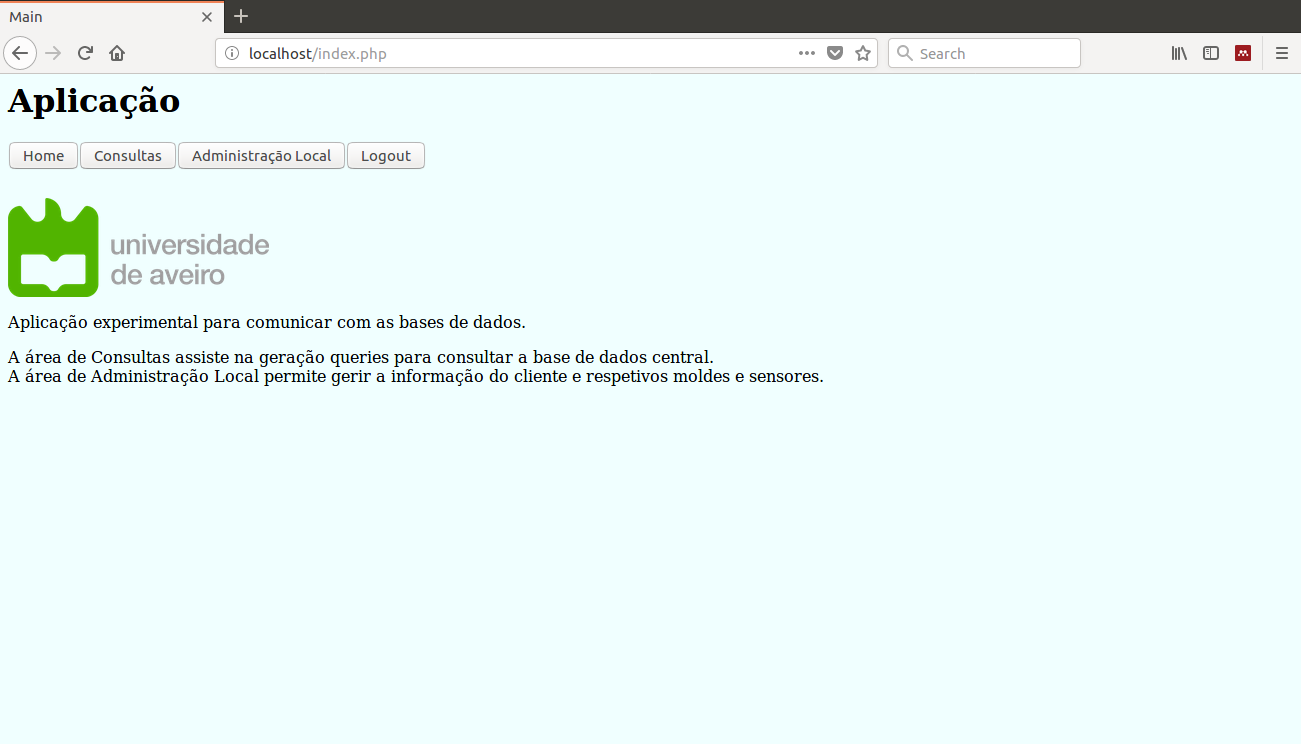
\includegraphics[width=0.85\textwidth]{main02} % Include the image placeholder.png
			\subcaption{Com \textit{login}}
			\label{fig:main2}
		\end{center}
	\end{minipage}
	\caption{Funcionalidades da página \textit{Main} com e sem \textit{login}}
	\label{fig:main0}
\end{figure}
\textit{Main} serve como página principal da aplicação. Se não houver sessão iniciada todas as restantes páginas redirecionam o utilizador para aqui. Contém apenas algumas informações gerais sobre a aplicação.\\
Iniciar sessão na página de \textit{Login} desbloqueia funcionalidades na aplicação, como demonstrado nas Figuras \ref{fig:main1} e \ref{fig:main2}. Depois de iniciada sessão navega-se com os botões para as páginas de Consultas, Administração e Conexão Local.

\subsection{\textit{Login}}
\begin{figure}[H]
	\begin{center}
		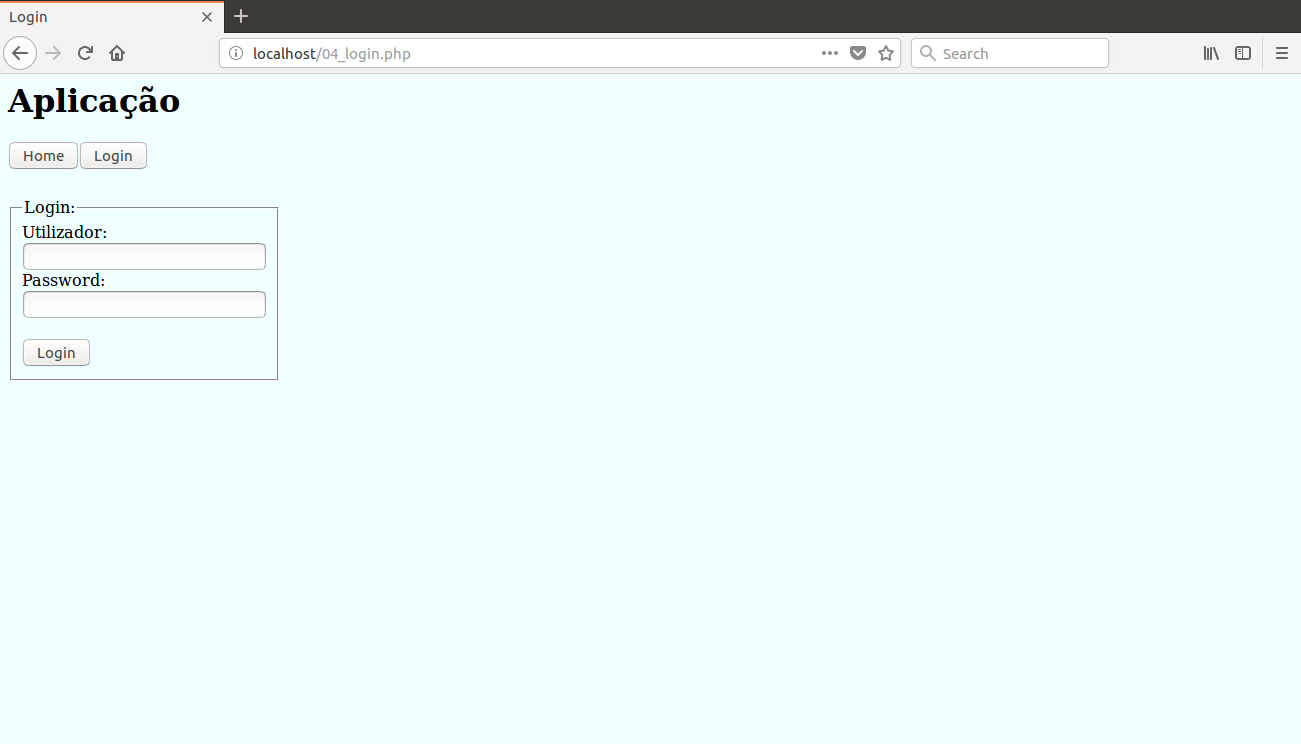
\includegraphics[width=0.9\textwidth]{login01} % Include the image placeholder.png
		\caption{Página de \textit{Login} para iniciar sessão na base de dados central}
		\label{fig:login0}
	\end{center}
\end{figure}
A página de \textit{Login} consiste num simples formulário constituído por duas caixas de texto e um botão, como demonstrado na \autoref*{fig:login0}. O botão \textit{Login} lê as credenciais introduzidas e realiza uma conexão de teste à base de dados central validando-as diretamente com \textit{MySQL}. Se as credenciais forem validadas com sucesso redireciona-se o utilizador para a página principal e altera-se o botão de \textit{Login} para \textit{Logout}. Se as credenciais introduzidas não forem suficientes ou válidas são retornados erros de forma a informar o utilizador como demonstrado nas Figuras \ref{fig:login2} e \ref{fig:login3}.\\
Quando se acede à página como \textit{Logout} termina-se a sessão e redireciona-se o utilizador para a página principal.
\begin{figure}[H]
	\centering
	\begin{minipage}{.5\textwidth}
		\begin{center}
			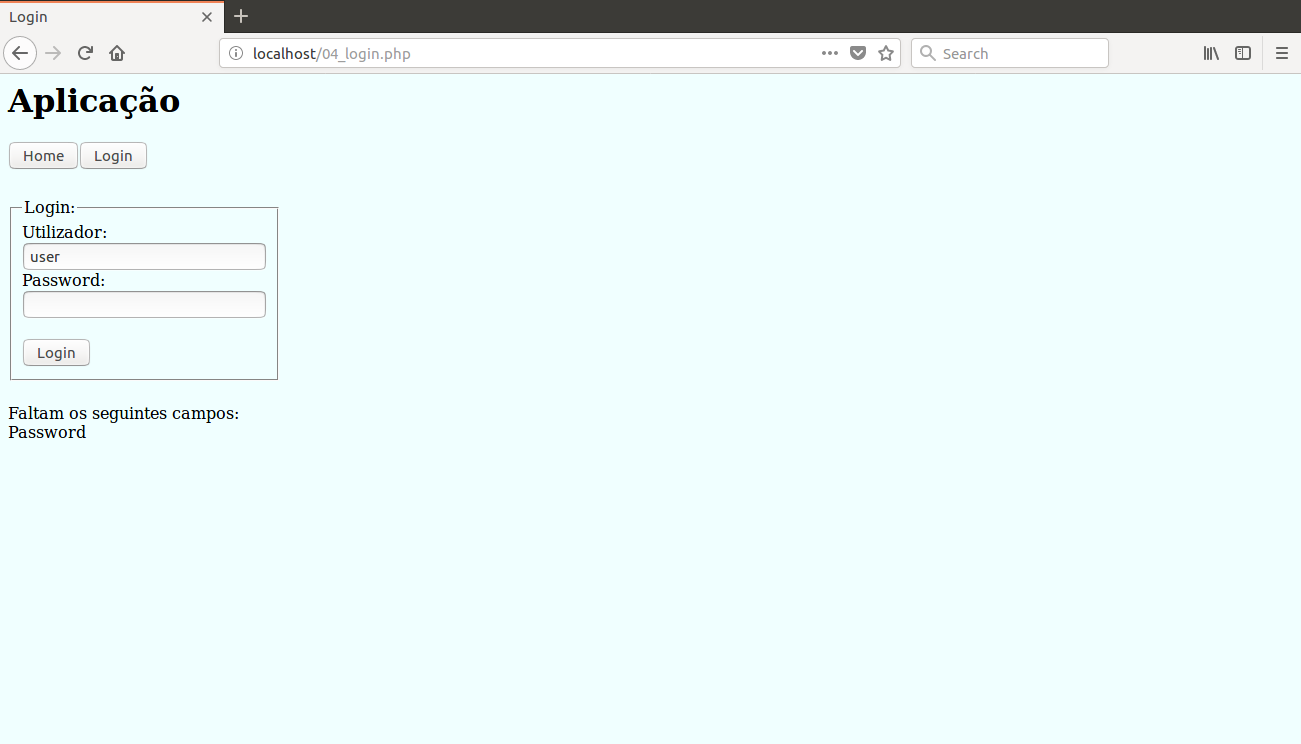
\includegraphics[width=0.95\textwidth]{login02} % Include the image placeholder.png
			\subcaption{Exemplo de erro de falta de informação}
			\label{fig:login2}
		\end{center}
	\end{minipage}%
	\begin{minipage}{.5\textwidth}
		\begin{center}
			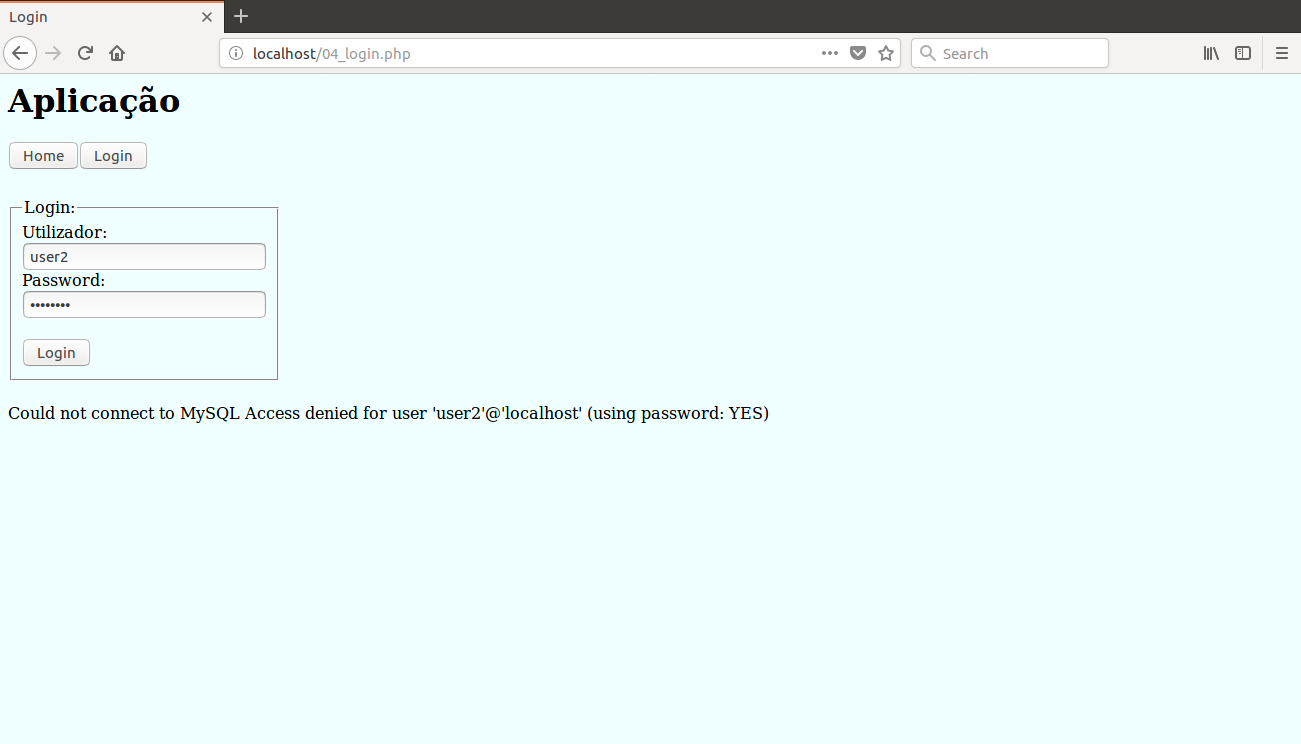
\includegraphics[width=0.95\textwidth]{login03} % Include the image placeholder.png
			\subcaption{Exemplo de erro \textit{MySQL}}
			\label{fig:login3}
		\end{center}
	\end{minipage}
	\caption{Exemplos de erros retornados quando introduzidas credenciais não válidas na página \textit{Login}}
	\label{fig:login1}
\end{figure}

\subsection{Consultas}
\begin{figure}[H]
	\centering
	\begin{minipage}{1.\textwidth}
		\begin{center}
			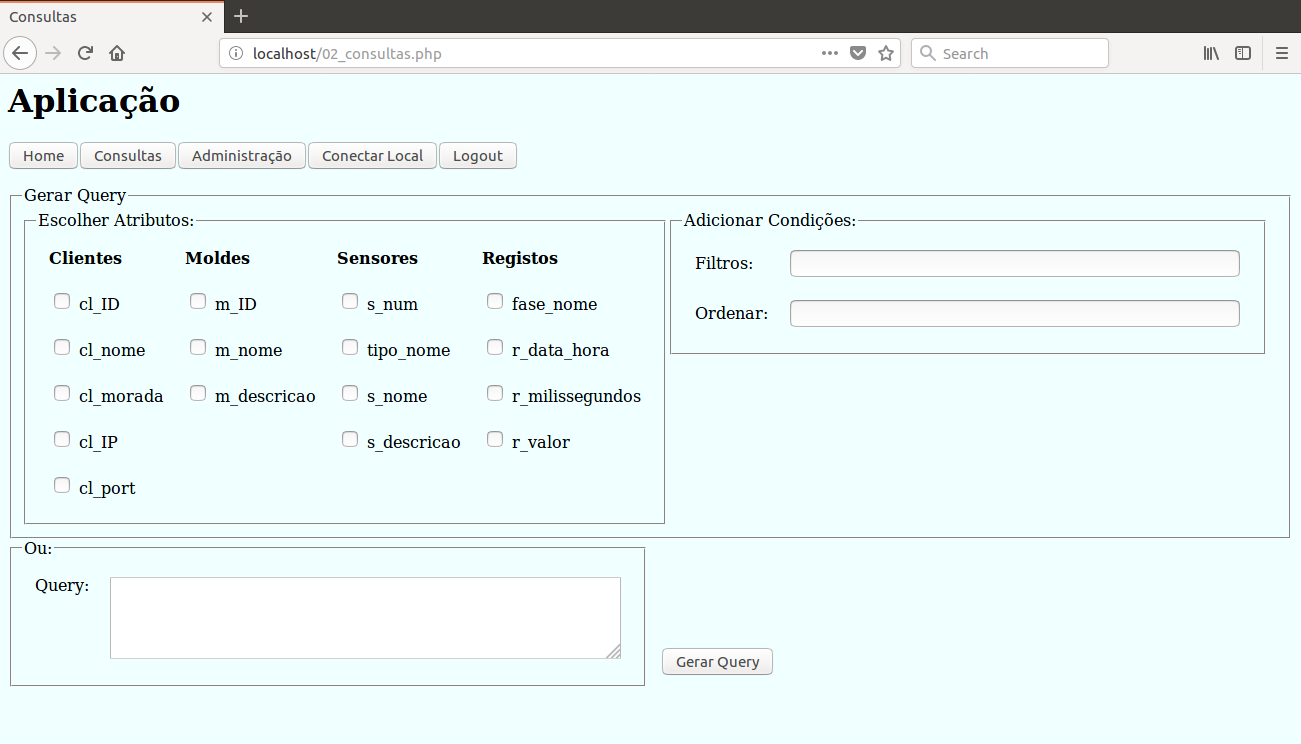
\includegraphics[width=.9\textwidth]{consultas01} % Include the image placeholder.png
			\subcaption{Página de Consultas}
			\label{fig:consultas1}
		\end{center}
	\end{minipage}
	\begin{minipage}{1.\textwidth}
		\begin{center}
			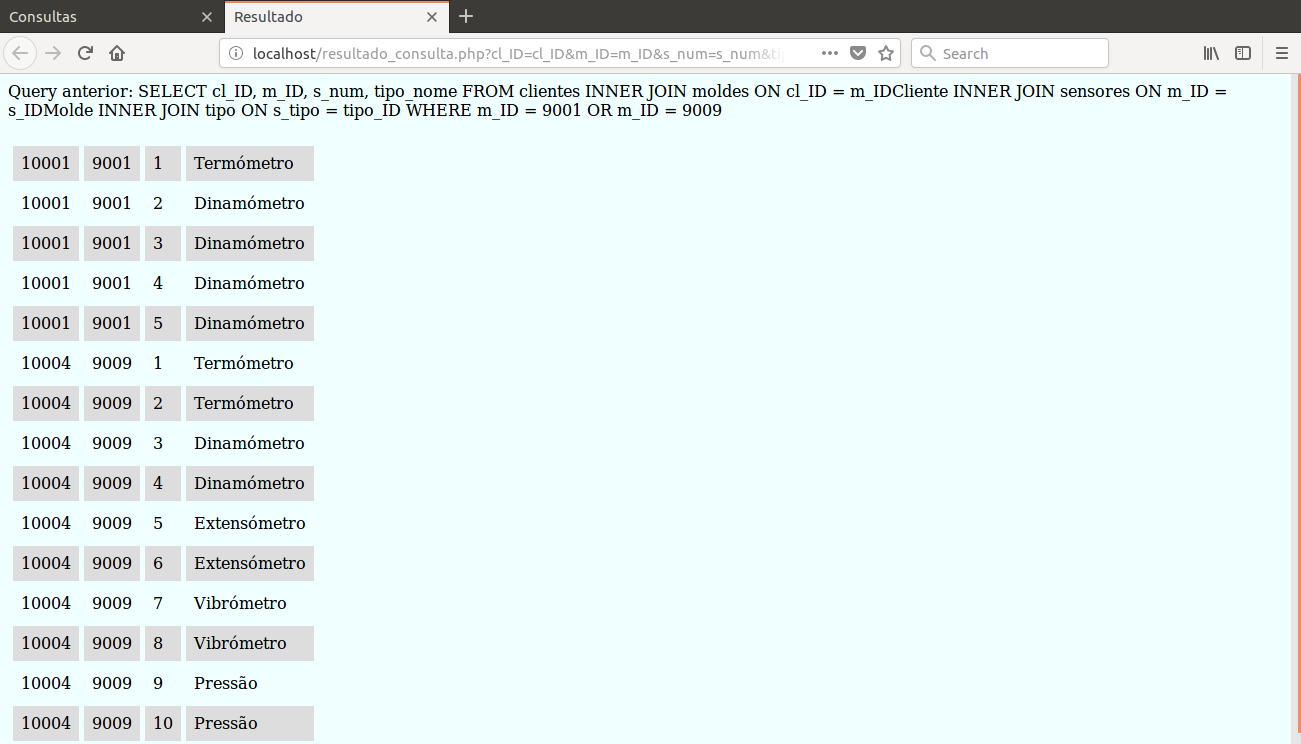
\includegraphics[width=0.9\textwidth]{consultas02} % Include the image placeholder.png
			\subcaption{Exemplo de resposta de consulta}
			\label{fig:consultas2}
		\end{center}
	\end{minipage}
	\caption{Página de Consultas e exemplo de resposta a uma consulta}
	\label{fig:consultas0}
\end{figure}
A página de Consultas assiste utilizadores sem conhecimentos de \textit{SQL} a criarem \textit{queries} para consultar a base de dados central. Na \autoref{fig:consultas1} observa-se várias \textit{checkboxes} e três caixas de texto. As \textit{checkboxes} permitem selecionar os atributos que se desejam consultar na base de dados, estes são guardados numa variável @atributos.
\newpage
Quando  se prime o botão \textit{Query} gera-se uma das seguintes \textit{queries}:
\begin{lstlisting}[language = SQL]
	SELECT @atributos
	FROM clientes;
	
	SELECT @atributos
	FROM clientes
	INNER JOIN moldes ON cl_ID = m_IDCliente;
	
	SELECT @atributos
	FROM clientes
	INNER JOIN moldes ON cl_ID = m_IDCliente
	INNER JOIN sensores ON m_ID = s_IDMolde
	INNER JOIN tipo ON s_tipo = tipo_ID;
	
	SELECT @atributos FROM clientes
	INNER JOIN moldes ON cl_ID = m_IDCliente
	INNER JOIN sensores ON m_ID = s_IDMolde 
	INNER JOIN tipo ON s_tipo = tipo_ID
	INNER JOIN registos ON s_IDMolde = r_IDMolde
	AND s_num = r_numSensor
	INNER JOIN fase ON r_fase = fase_ID;
\end{lstlisting}
Efetua-se esta seleção com base na coluna mais à esquerda a que os atributos pertencem. Explicando melhor com um exemplo: se o utilizador desejar consultar o cl\texttt{\char`_}ID e o cl\texttt{\char`_}nome da tabela clientes gera-se a primeira \textit{query} no entanto, se o utilizador desejar consultar os atributos cl\texttt{\char`_}ID, m\texttt{\char`_}ID e s\texttt{\char`_}num gera-se a terceira \textit{query}.\\
Além destas, existem três \textit{queries} especificas quando os atributos tipo\texttt{\char`_}nome, fase\texttt{\char`_}nome e r\texttt{\char`_}data\texttt{\char`_}hora são selecionados sozinhos. As primeiras duas permitem consultar as opções disponíveis nos dicionários e a terceira devolve as datas e horas entre o primeiro e último registos.\\
As caixas de texto Filtros e Ordem permitem adicionar às \textit{queries} geradas as cláusulas WHERE e ORDER BY, respetivamente. Para os utilizadores com conhecimentos em \textit{SQL} está disponibilizada a caixa de texto \textit{Query} que permite a criação direta de uma \textit{query}. Este campo está limitado apenas para \textit{queries} do tipo SELECT.\\
Depois da \textit{query} ser gerada retorna-se uma resposta num novo separador como demonstrado na \autoref{fig:consultas2}. O \textit{link} deste resposta contém toda a informação da \textit{query} gerada. Este pode ser arquivado ou enviado para outro utilizador sem ser necessário gerar a \textit{query} novamente, isto é útil para \textit{queries} com muitas cláusulas.\\
Se a \textit{query} não for válida retorna-se um erro de forma a informar o utilizador, como demonstrado nas Figuras \ref{fig:consultas4}, \ref{fig:consultas5} e \ref{fig:consultas6}.
\newpage
\begin{figure}[H]
	\centering
	\begin{minipage}{1\textwidth}
		\begin{center}
			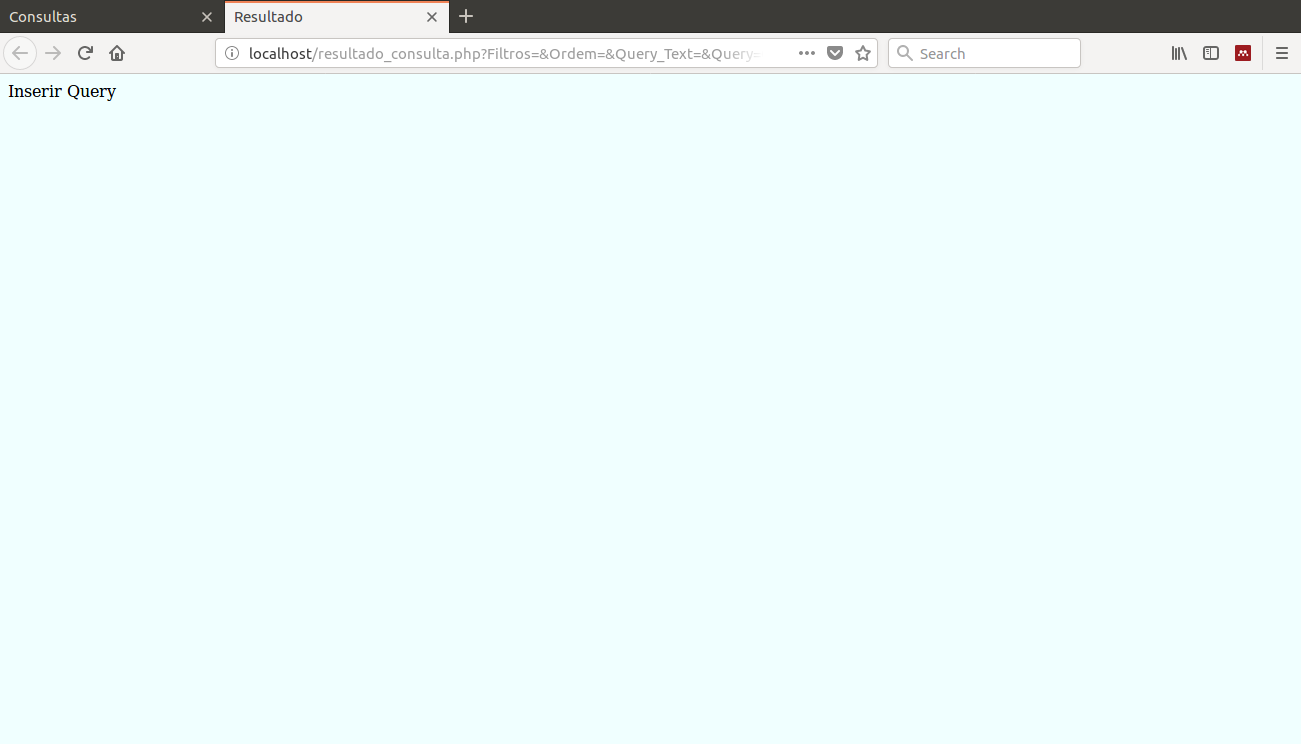
\includegraphics[width=0.7\textwidth]{consultas03} % Include the image placeholder.png
			\subcaption{Erro de informação não introduzida}
			\label{fig:consultas4}
		\end{center}
	\end{minipage}
	\begin{minipage}{1\textwidth}
		\begin{center}
			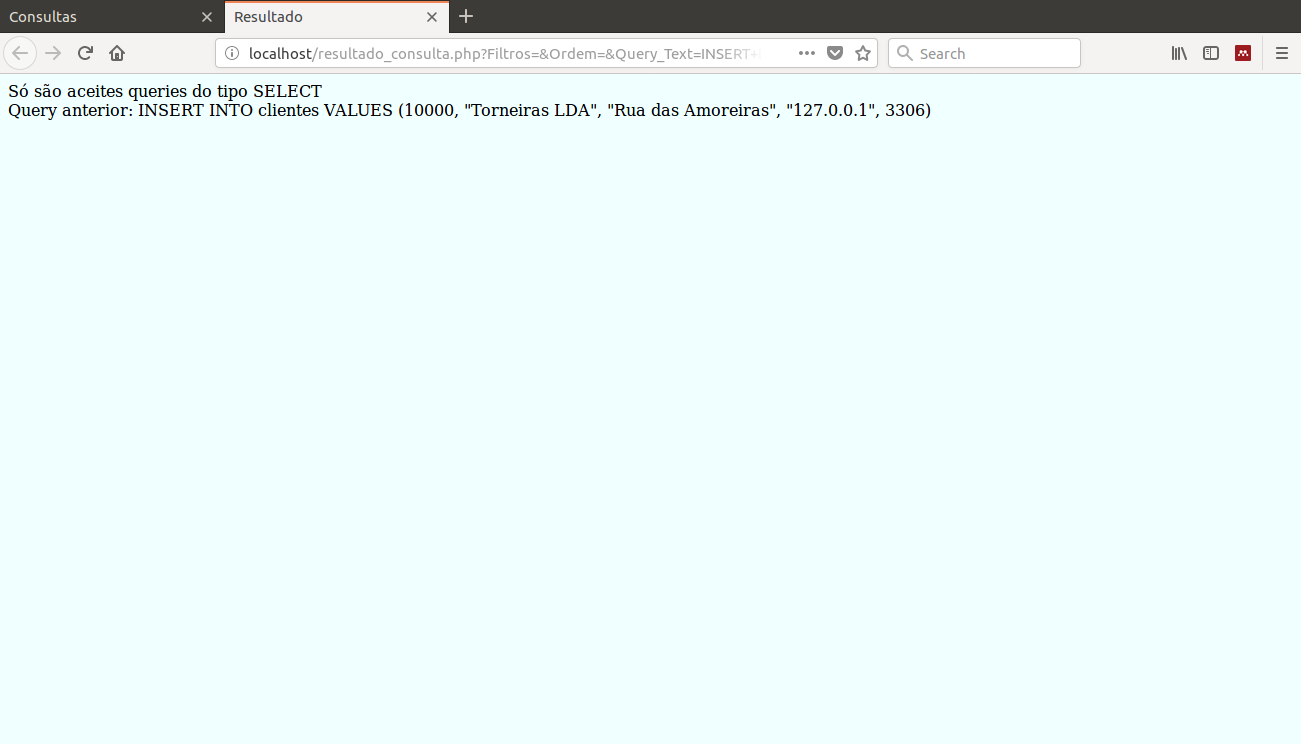
\includegraphics[width=0.7\textwidth]{consultas04} % Include the image placeholder.png
			\subcaption{Erro de \textit{query} que não é do tipo SELECT}
			\label{fig:consultas5}
		\end{center}
	\end{minipage}
	\begin{minipage}{1\textwidth}
		\begin{center}
			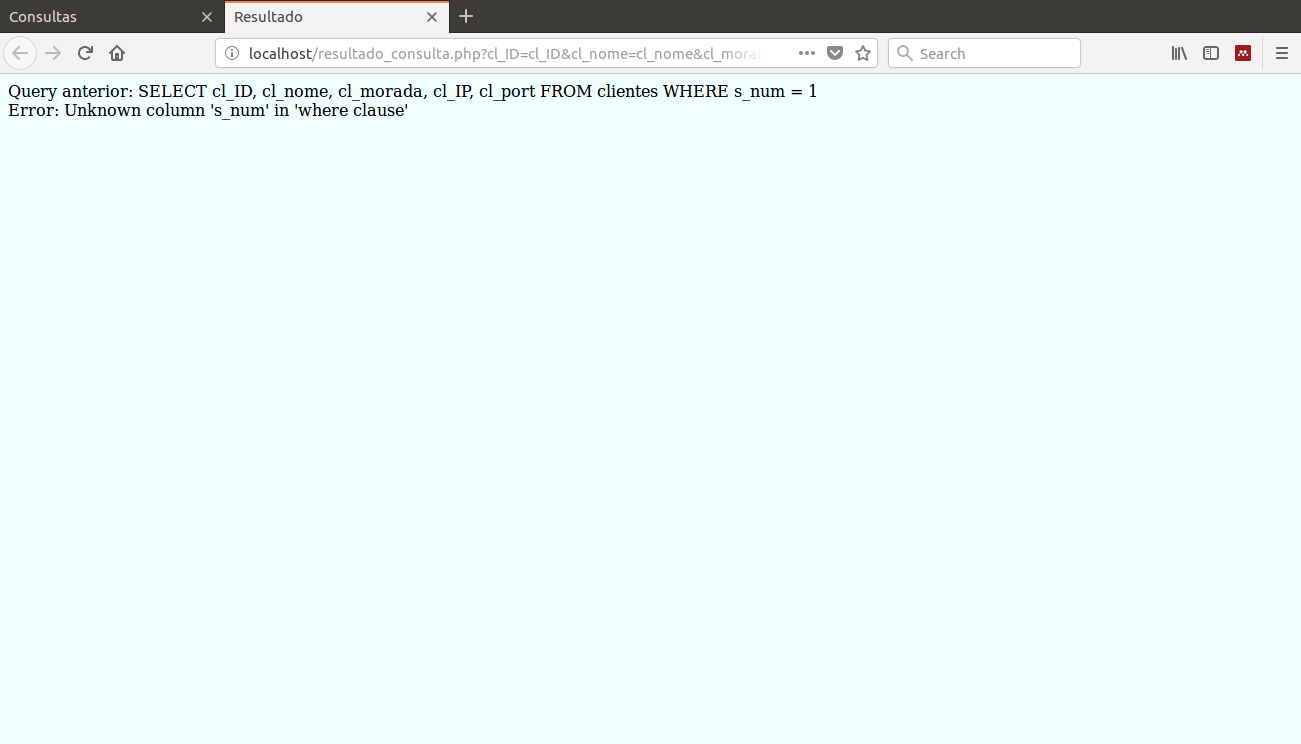
\includegraphics[width=0.7\textwidth]{consultas05} % Include the image placeholder.png
			\subcaption{Exemplo de erro \textit{MySQL}}
			\label{fig:consultas6}
		\end{center}
	\end{minipage}
	\caption{Exemplos de erros retornados na página de Resposta da Consulta}
	\label{fig:consultas3}
\end{figure}

\subsection{Administração}
\begin{figure}[H]
	\centering
	\begin{minipage}{1\textwidth}
		\begin{center}
			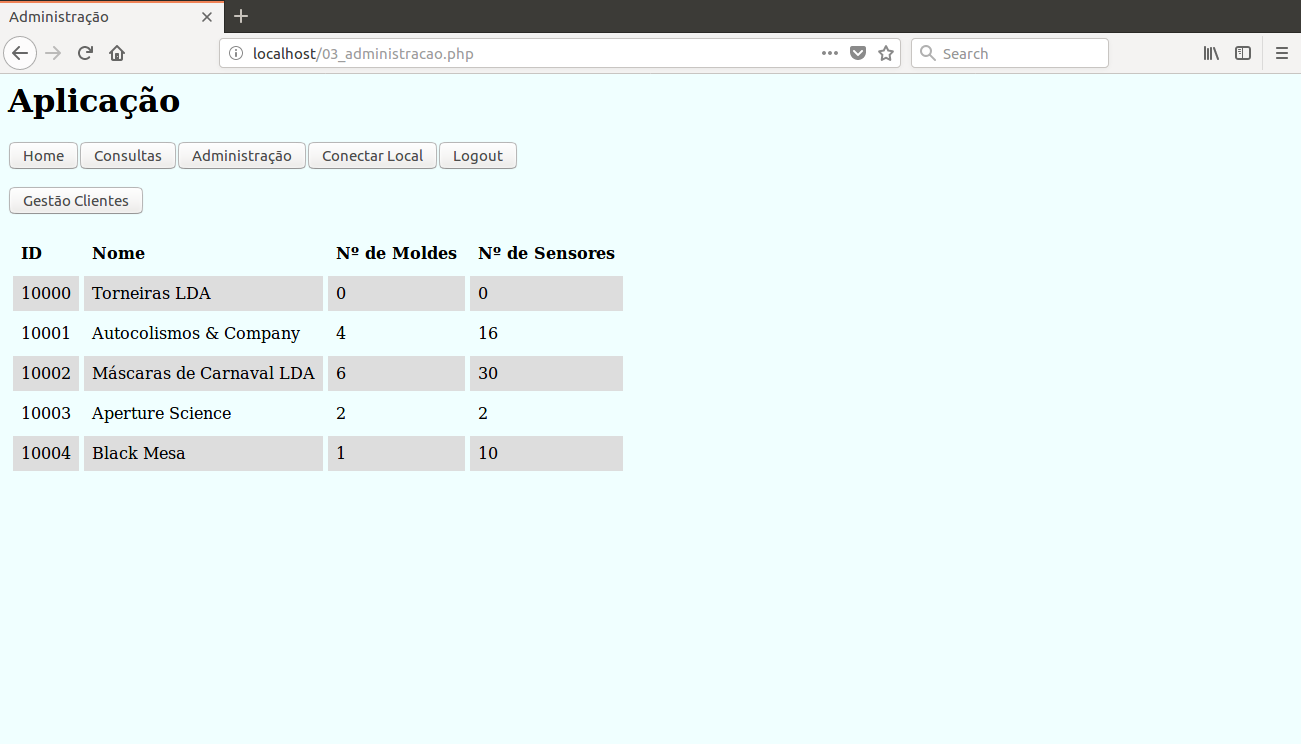
\includegraphics[width=0.9\textwidth]{administracao01} % Include the image placeholder.png
			\subcaption{Sem conexão local}
			\label{fig:admin1}
		\end{center}
	\end{minipage}
	\begin{minipage}{1\textwidth}
		\begin{center}
			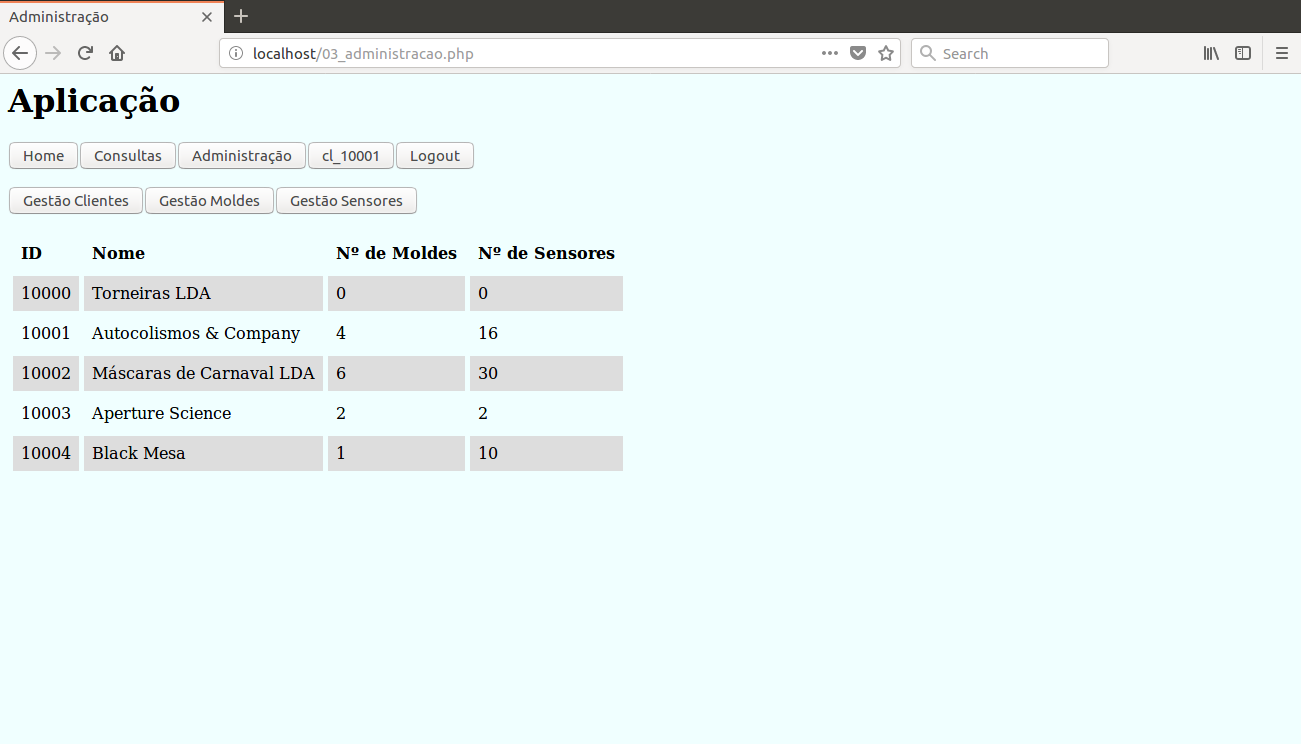
\includegraphics[width=0.9\textwidth]{administracao03} % Include the image placeholder.png
			\subcaption{Com conexão local}
			\label{fig:admin2}
		\end{center}
	\end{minipage}
	\caption{Funcionalidades da página Administração com e sem conexão local}
	\label{fig:admin0}
\end{figure}
\newpage
A área de Administração permite ao utilizador alterar informações sobre os clientes, moldes e sensores. A partir de qualquer dispositivo só é possível aceder à Gestão de Clientes como demonstrado na \autoref{fig:admin1}. Nesta área a informação dos clientes pode ser alterada com o formulário demonstrado na \autoref{fig:admin3}. Os botões Adicionar Cliente, Alterar Cliente e Eliminar Cliente executam \textit{queries} do tipo INSERT, UPDATE e DELETE, respetivamente.\\
\\
\\
\\
\\
\\
\\
\\
\\
\\
\\
\begin{figure}[H]
	\begin{center}
		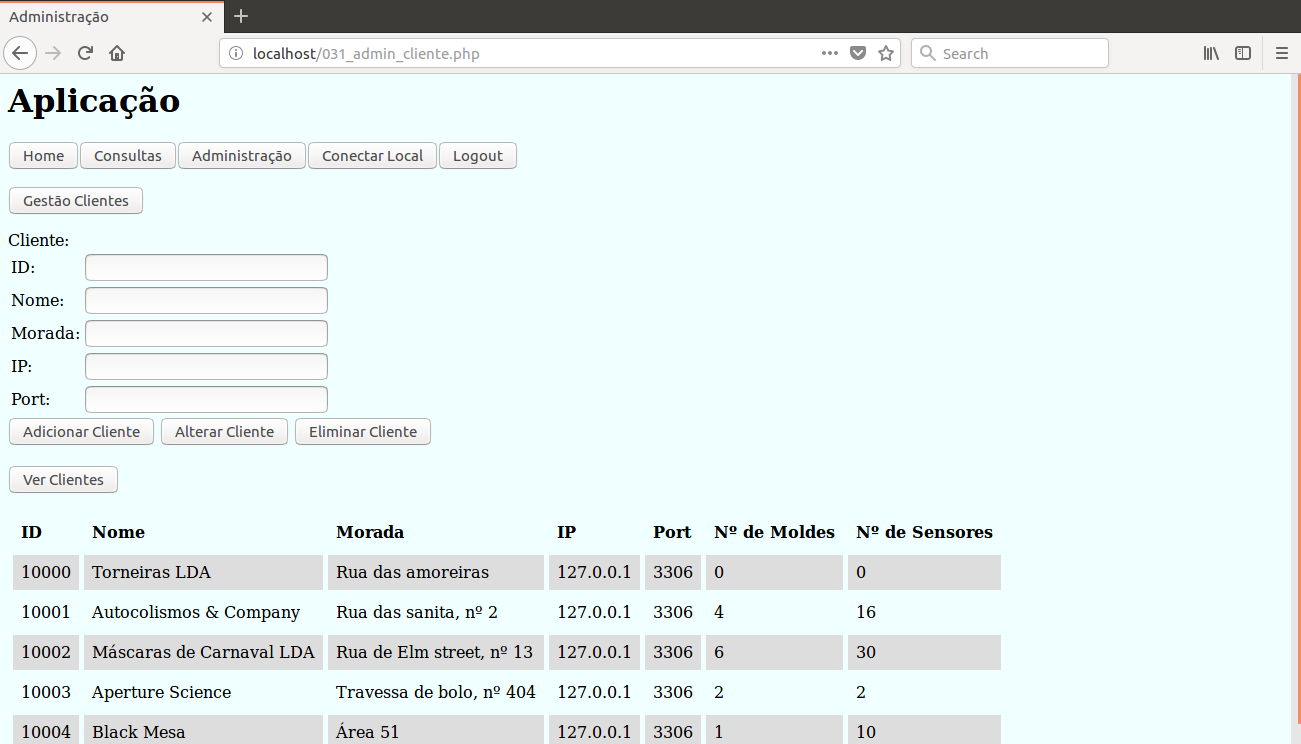
\includegraphics[width=0.9\textwidth]{administracao02} % Include the image placeholder.png
		\caption{Área de Gestão de Clientes sem conexão local}
		\label{fig:admin3}
	\end{center}
\end{figure}
\newpage
Como referido anteriormente a aplicação divide-se numa utilização geral e local, todas as funcionalidades descritas até agora têm em vista uma utilização geral. As restantes funcionalidades que são descritas até ao final do capítulo visam um uso local.\\
Após uma conexão bem sucedida ao sistema local do cliente são desbloqueadas novas áreas de gestão como mostra a \autoref{fig:admin2}. As áreas de Gestão de Moldes e Gestão de Sensores demonstradas nas Figuras \ref{fig:admin9} e \ref{fig:admin10}, permitem ao utilizador criar e apagar moldes e sensores, respetivamente. Estes dados são inseridos na base de dados temporária local, aqui o utilizador pode criar e apagar moldes e sensores sem afetar o sistema. Desta forma é possível confirmar a informação introduzida antes de a inserir no sistema. Os botões de Criar e Apagar nestes formulários realizam \textit{queries} do tipo INSERT e DELETE, respetivamente.
	\begin{figure}[H]
		\centering
			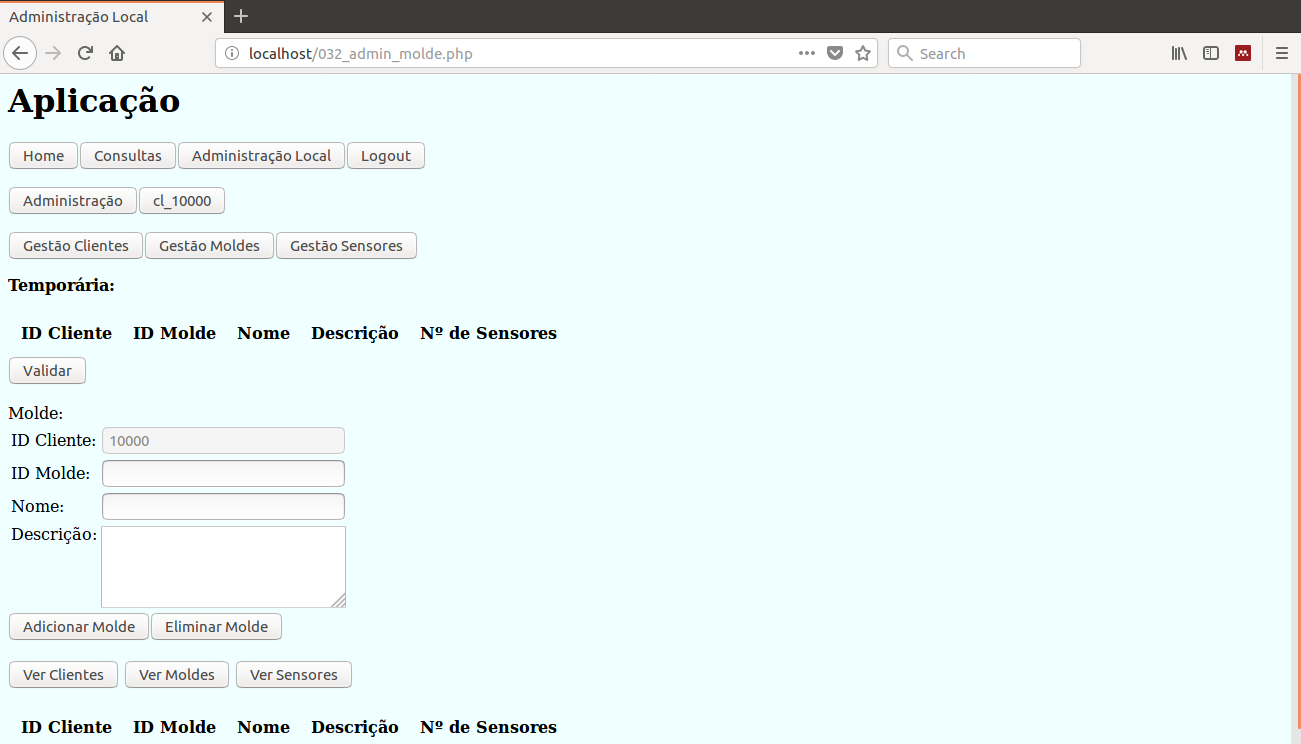
\includegraphics[width=0.8\textwidth]{administracao05} % Include the image placeholder.png
			\caption{Área de Gestão de Moldes}
			\label{fig:admin9}
	\end{figure}
	\begin{figure}[H]
		\centering
			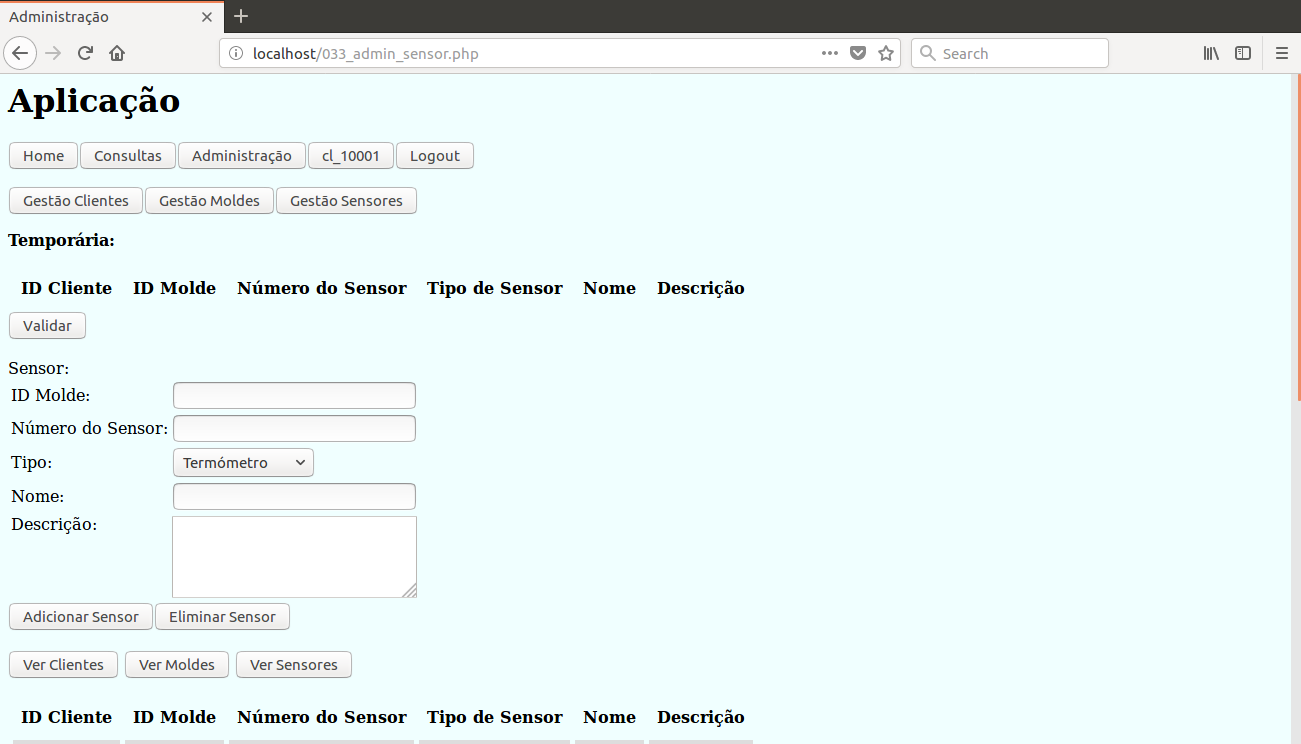
\includegraphics[width=0.8\textwidth]{administracao06} % Include the image placeholder.png
			\caption{Área de Gestão de Sensores}
			\label{fig:admin10}
	\end{figure}
Quando a informação dos moldes e sensores estiver completa o botão Validar tenta registar os valores presentes na base de dados temporária local nas bases de dados central e local. Se a ação não executar com sucesso é retornado um erro \textit{MySQL} de forma a informar o utilizador. Se a ação executar com sucesso a base de dados temporária local é limpa e os valores são registados permanentemente nas bases de dados central e local, como representado nas Figuras \ref{fig:admin12} e \ref{fig:admin13}.\\
Depois de inseridos, moldes e sensores, não podem ser eliminados via aplicação. Esta opção foi removida da aplicação para evitar erros, dado que apagar um molde em funcionamento faz com que se percam novos registos.
\begin{figure}[H]
	\centering
	\begin{minipage}{.5\textwidth}
		\begin{center}
			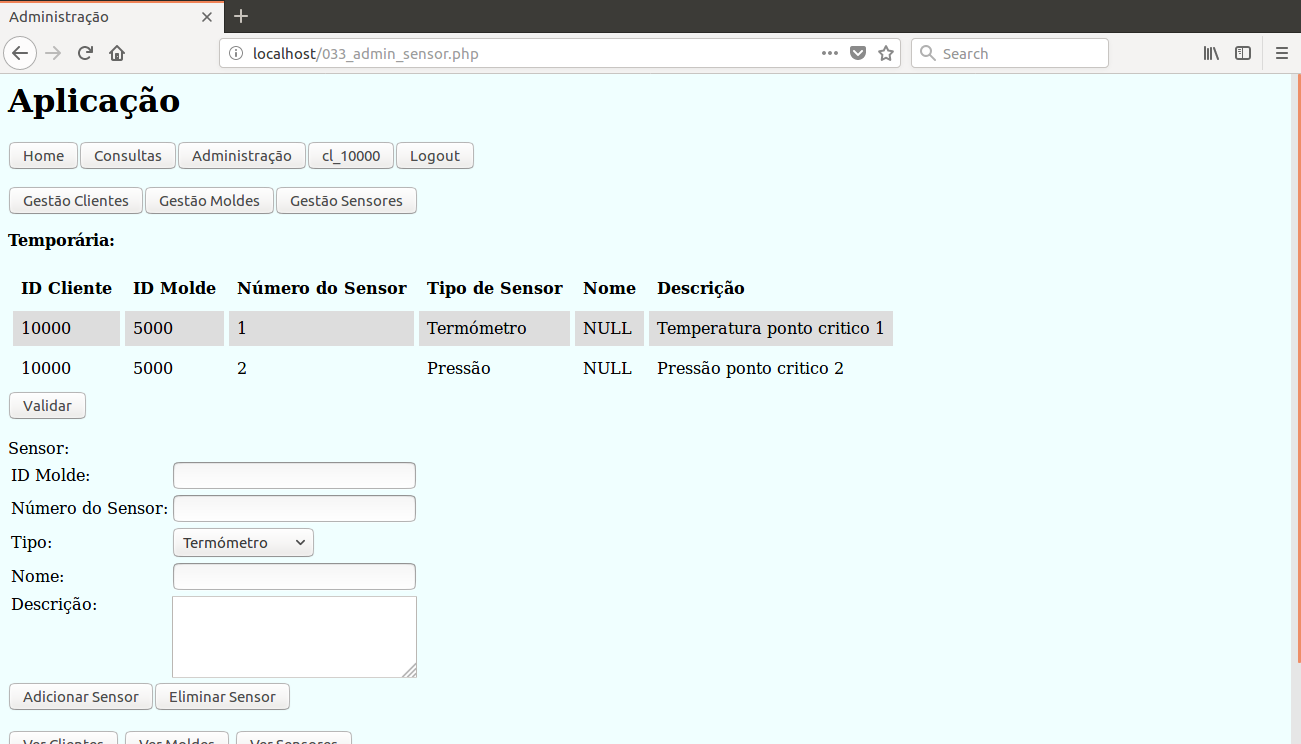
\includegraphics[width=0.9\textwidth]{administracao07} % Include the image placeholder.png
			\subcaption{Dados antes de serem validados}
			\label{fig:admin12}
		\end{center}
	\end{minipage}%
	\begin{minipage}{.5\textwidth}
		\begin{center}
			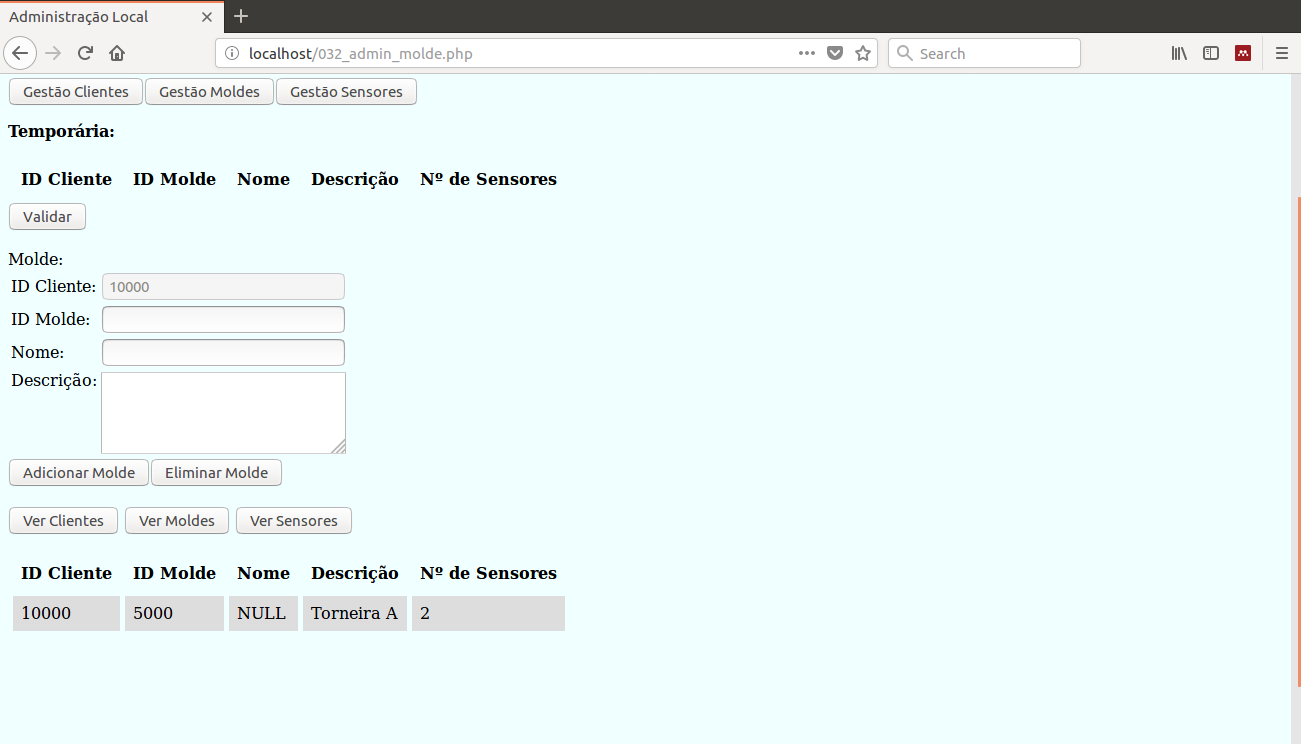
\includegraphics[width=0.9\textwidth]{administracao08} % Include the image placeholder.png
			\subcaption{Dados após serem validados}
			\label{fig:admin13}
		\end{center}
	\end{minipage}
	\caption{Função do botão Validar, onde os valores da base de dados temporária local são transferidos de forma permanente para as bases de dados central e local}
	\label{fig:admin11}
\end{figure}
Voltando a área de Gestão de Clientes, após a conexão local, desbloqueia-se uma nova funcionalidade como demonstra a \autoref{fig:admin7}. O botão Atualizar permite reiniciar o programa de transferência de valores para que este atualize o número de clientes. Com o comando:
\begin{lstlisting}[language = bash]
	ps ax | grep transferencia
\end{lstlisting}
Obtém-se os números de processo dos programas que estão a transferir valores. Estes valores são armazenados na variável @pids. Para terminar os programas utiliza-se o seguinte comando:
\begin{lstlisting}[language = bash]
	kill -2 @pids
\end{lstlisting}
A opção -2 permite enviar para o processo escolhido o sinal SIGINT que é o sinal esperado pelo programa para que este termine as suas rotinas antes de encerrar. Para iniciar novamente o comando usar:
\begin{lstlisting}[language = bash]
	~/path/transferencia
\end{lstlisting}
É necessário garantir permissões ao servidor \textit{Apache} no sistema central para que este possa executar estes comandos.
\newpage
\begin{figure}[H]
	\centering
			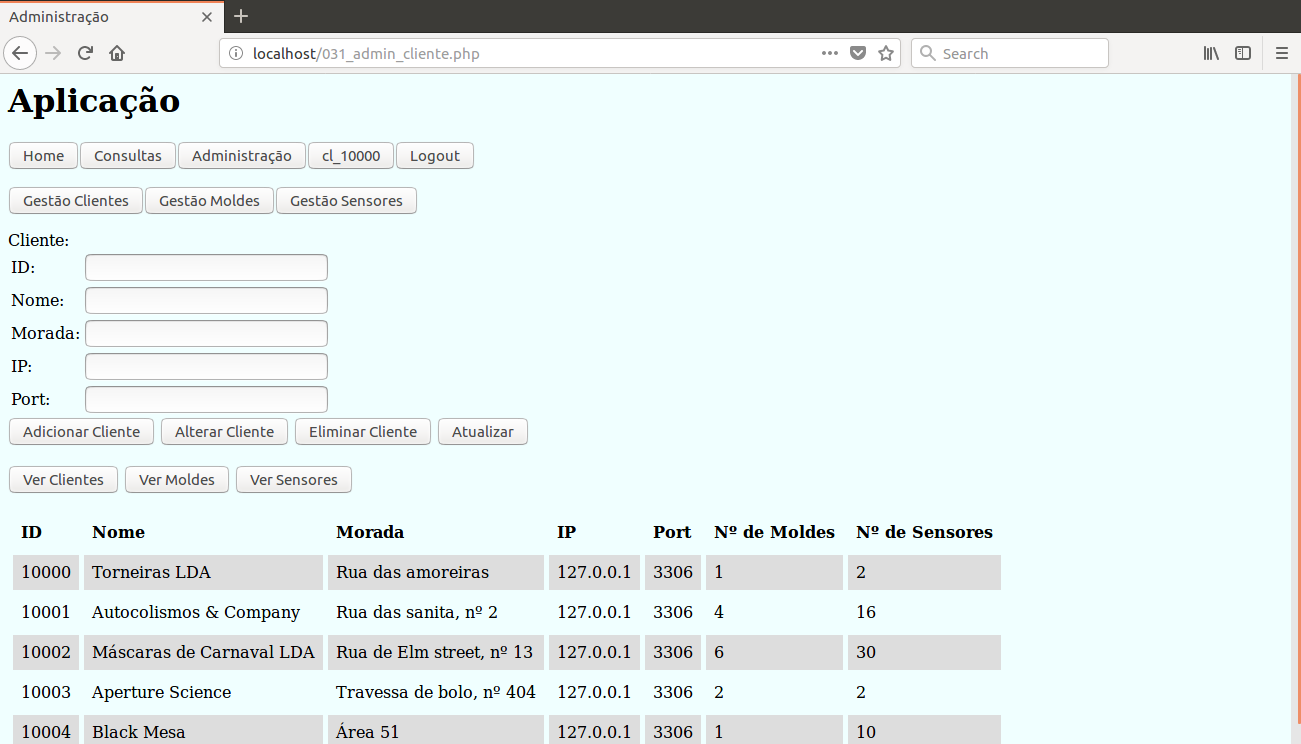
\includegraphics[width=0.9\textwidth]{administracao04} % Include the image placeholder.png
	\caption{Área de Gestão de Clientes após conexão local onde se visualiza o botão Atualizar}
	\label{fig:admin7}
\end{figure}
Nas várias áreas de gestão existem os botões Ver Clientes, Ver Moldes e Ver Sensores que executam respetivamente as \textit{queries}:
\begin{lstlisting}[language = SQL]
	SELECT cl_ID, cl_nome, cl_morada, cl_IP, cl_port,
	COUNT(DISTINCT m_ID), COUNT(DISTINCT s_IDMolde, s_num)
	FROM clientes
	LEFT OUTER JOIN moldes ON cl_ID = m_IDCliente
	LEFT OUTER JOIN sensores ON m_ID = s_IDMolde
	GROUP BY cl_ID
	ORDER BY cl_ID
	
	SELECT m_IDCliente, m_ID, m_nome, m_descricao,
	COUNT(DISTINCT s_IDMolde, s_num)
	FROM clientes
	INNER JOIN moldes ON cl_ID = m_IDCliente
	LEFT OUTER JOIN sensores ON m_ID = s_IDMolde
	GROUP BY m_ID
	ORDER BY m_IDCliente, m_ID
	
	SELECT m_IDCliente, s_IDMolde, s_num, tipo_nome,
	s_nome, s_descricao
	FROM moldes
	INNER JOIN sensores ON m_ID = s_IDMolde
	INNER JOIN tipo ON s_tipo = tipo_id
	ORDER BY m_IDCliente, s_IDMolde, s_num
\end{lstlisting}
Estas fornecem algumas informações contextuais para facilitar a navegação do utilizador.

\subsection{Conexão local}
\label{subchap:local}
	\begin{figure}[H]
		\centering
			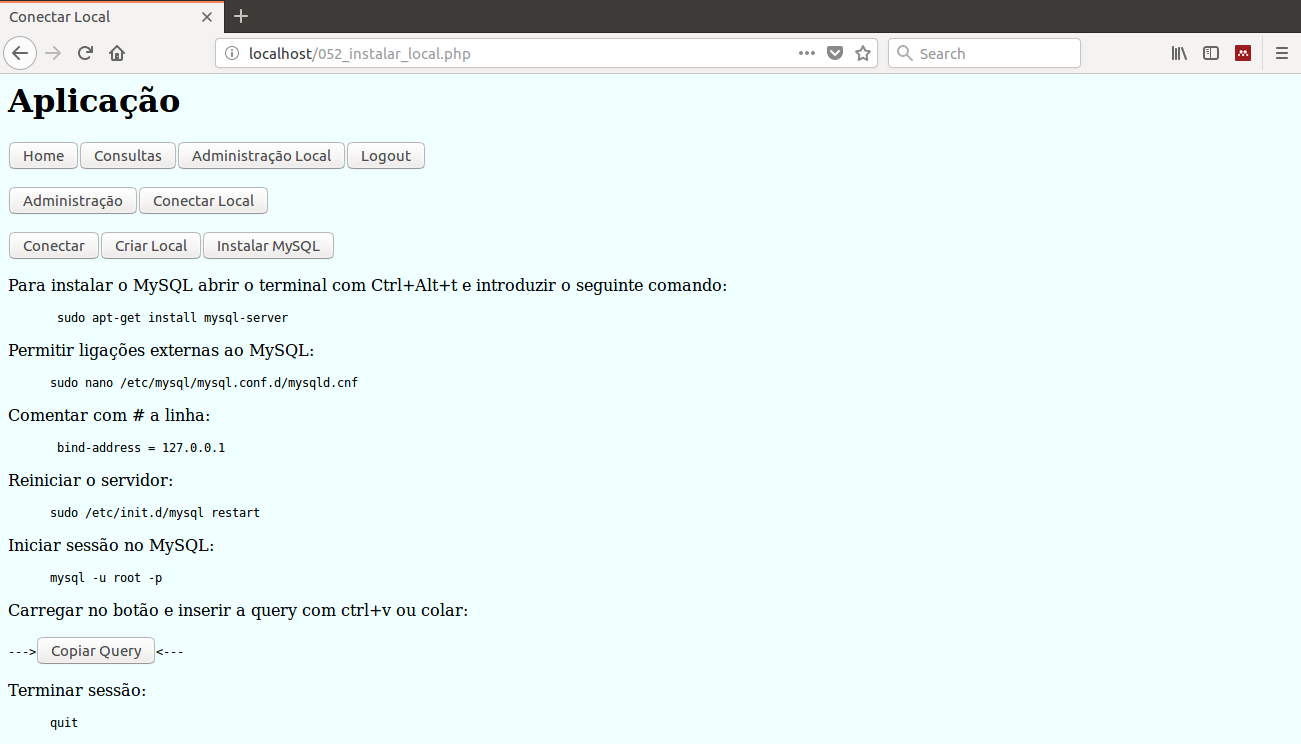
\includegraphics[width=0.9\textwidth]{local01} % Include the image placeholder.png
			\caption{Área Conectar Local onde se visualiza as bases de dados instaladas no sistema}
			\label{fig:local1}
	\end{figure}
A área de Conectar Local na \autoref{fig:local1} permite realizar uma conexão à base de dados local no servidor do cliente. Com recurso à \textit{query}:
\begin{lstlisting}[language = SQL]
	SHOW DATABASES
\end{lstlisting}
Obtém-se todas as bases de dados instaladas no servidor local. Do ponto de vista prático, cada cliente só terá uma base de dados local mas, para efeitos de desenvolvimento do projeto adotou-se esta vertente.
O botão Conectar inicia sessão na base de dados local escolhida e redireciona o utilizador para a página principal como se observar na \autoref{fig:local4}. O botão Desconectar termina esta sessão e redireciona o utilizador também, para a página principal.
\newpage
\begin{figure}[H]
	\begin{center}
		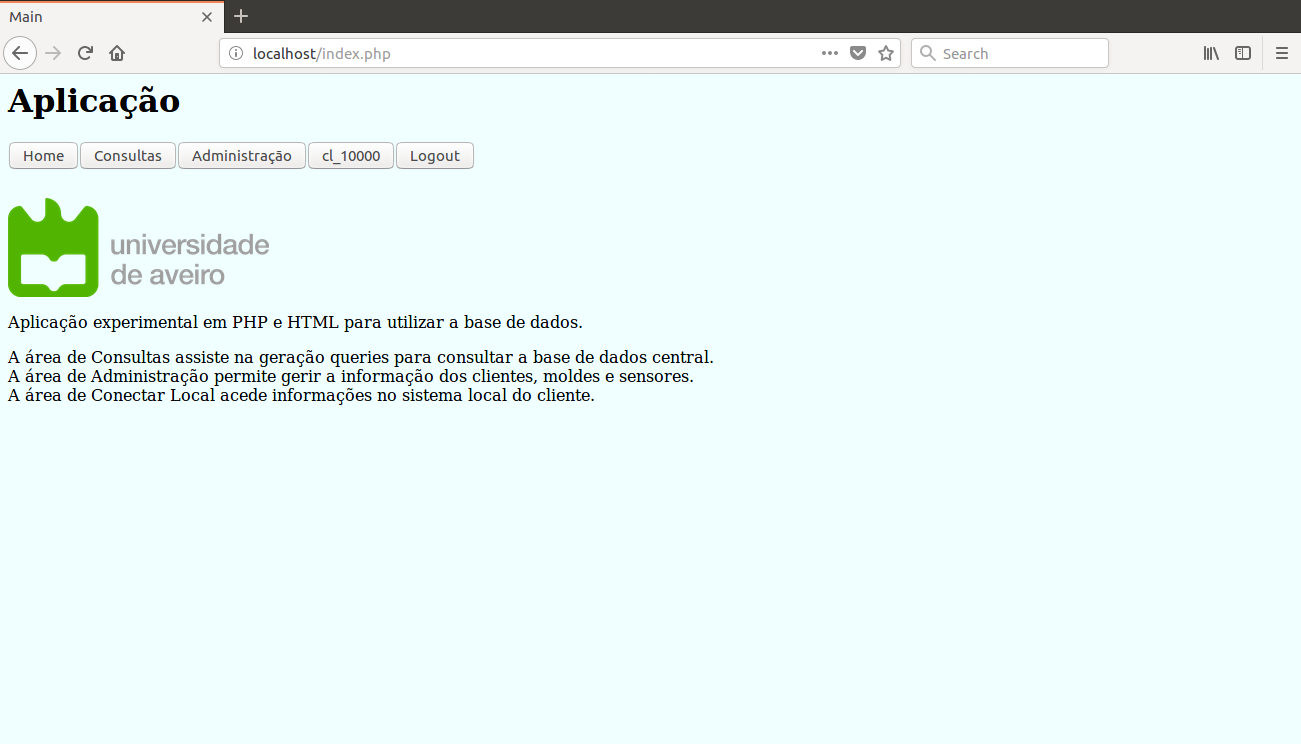
\includegraphics[width=0.9\textwidth]{main03} % Include the image placeholder.png
		\caption{\textit{Main} com conexão local}
		\label{fig:local4}
	\end{center}
\end{figure}
	\begin{figure}[H]
		\centering
		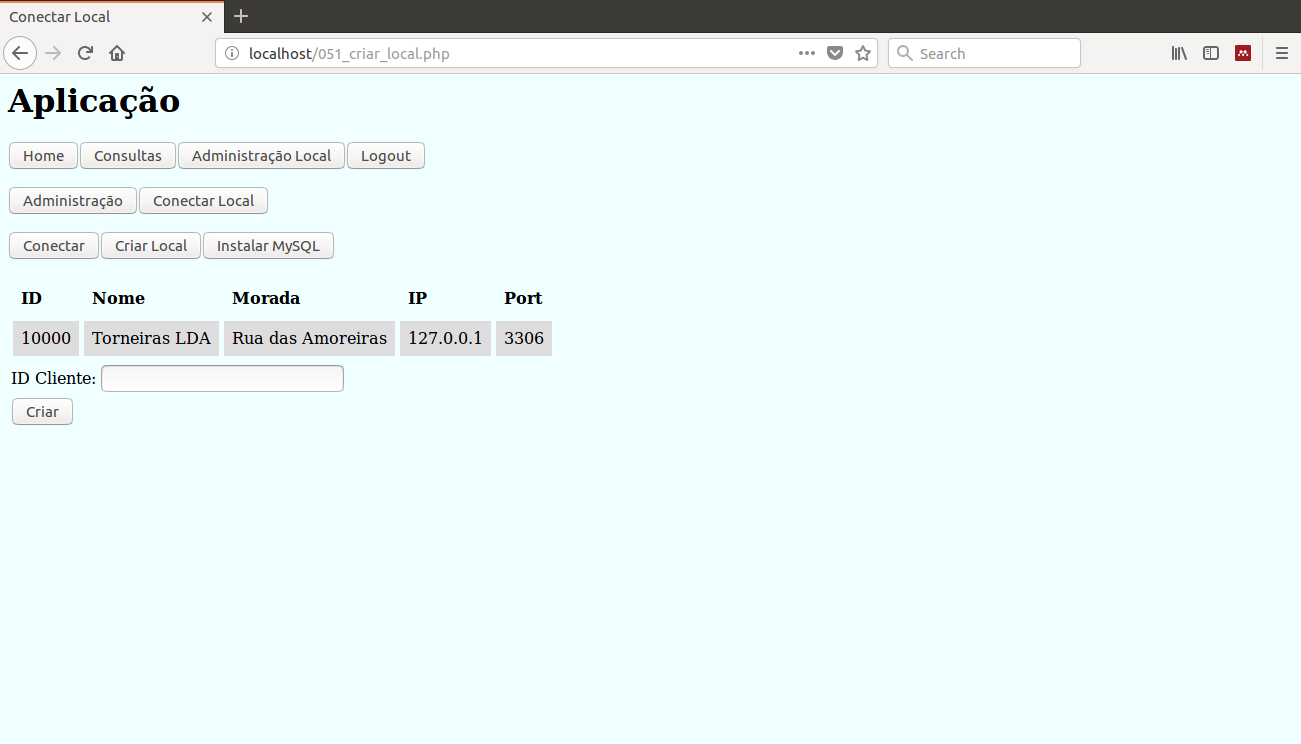
\includegraphics[width=0.9\textwidth]{local02} % Include the image placeholder.png
		\caption{Área Criar Local cria a base de dados para o cliente selecionado no sistema em que se acede a aplicação}
		\label{fig:local2}
	\end{figure}
A área Criar Local na \autoref{fig:local2} permite instalar uma base de dados para um novo cliente. São considerados novos clientes todos os que não tenham moldes associados a si, esta informação obtém-se com a \textit{query}:
\newpage
\begin{lstlisting}[language = SQL]
	SELECT cl_ID, cl_nome, cl_morada, cl_IP, cl_port
	FROM
		(SELECT cl_ID, cl_nome, cl_morada, cl_IP, cl_port,
		COUNT(DISTINCT m_ID) AS n_moldes
		FROM clientes
		LEFT OUTER JOIN moldes ON cl_ID = m_IDCliente
		GROUP BY cl_ID) AS contagem
	WHERE n_moldes = 0
\end{lstlisting}
Escolhendo um cliente válido o botão Criar cria a base de dados local com as respetivas tabelas e gera ainda as \textit{queries} observadas na \autoref{fig:local5}.
\begin{figure}[H]
	\begin{center}
		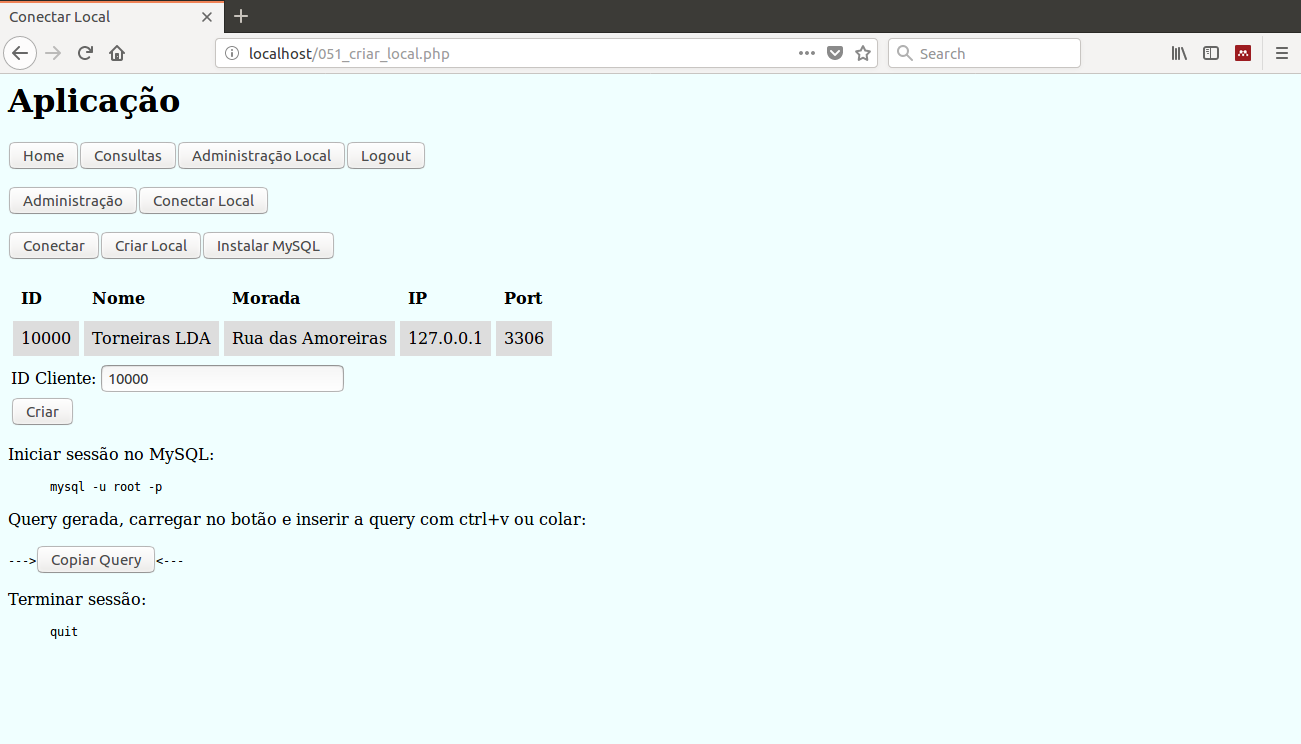
\includegraphics[width=0.9\textwidth]{local03} % Include the image placeholder.png
		\caption{\textit{Queries} geradas para completar a instalação da base de dados no sistema local. Consistem nas permissões para os utilizadores que só podem ser garantidas via \textit{root} bem como informação para completar o sistema de dados}
		\label{fig:local5}
	\end{center}
\end{figure}
\newpage
Terminado a análise das funcionalidades da aplicação com a área de Instalar \textit{MySQL} na \autoref{fig:local3} que contém os passos para instalar o \textit{MySQL} num sistema \textit{Linux}.
\begin{figure}[H]
	\centering
	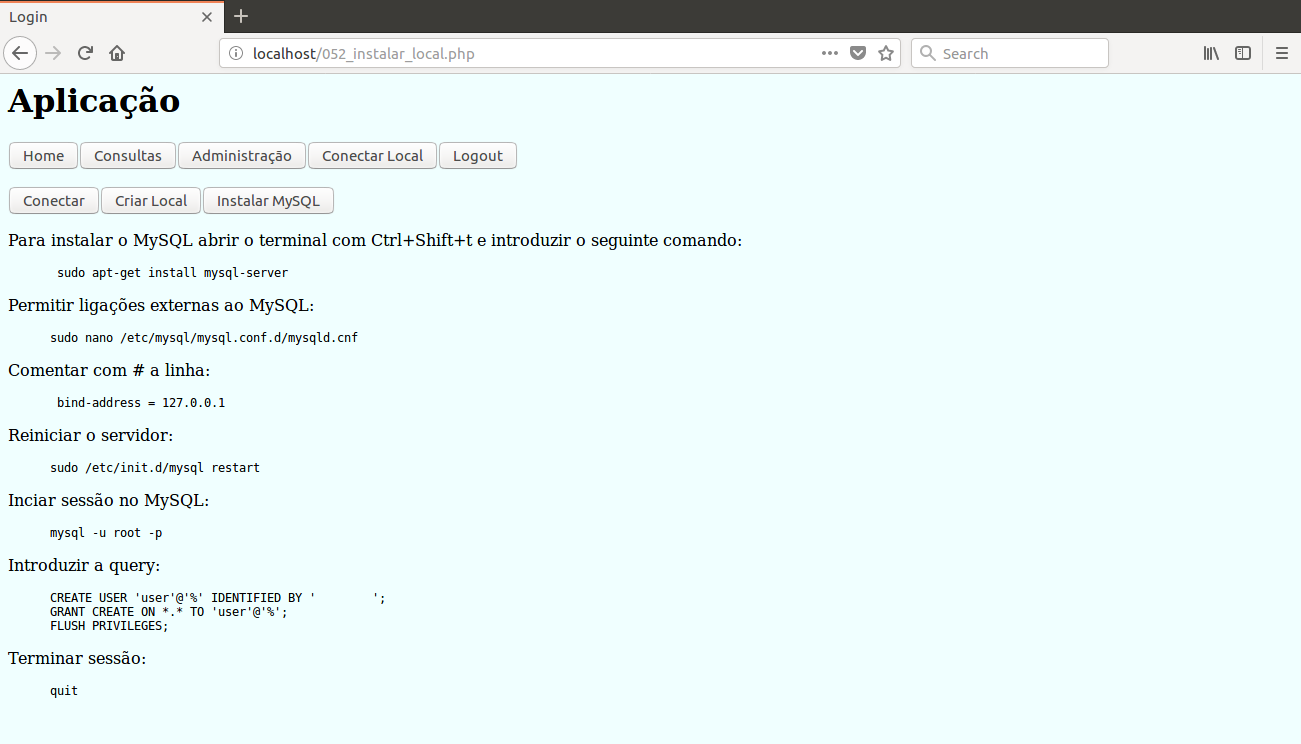
\includegraphics[width=0.9\textwidth]{local04} % Include the image placeholder.png
	\caption{Área Instalar \textit{MySQL} para instalar o \textit{software} com os comandos em \textit{Linux}}
	\label{fig:local3}
\end{figure}

%\cleardoublepage
%\chapter{Instalação do Sistema}

\cleardoublepage
\chapter{Conclusões}
O desafio proposto consiste em monitorizar sensores remotamente. Para isto definiu-se como objetivos principais desenvolver uma rede de bases de dados e uma aplicação que permitisse interagir com estas. Estes objetivos foram concluídos com sucesso. Este capítulo contém comentários sobre o desempenho da solução desenvolvida e propostas para trabalhos futuros.

\section{Comentários}
\subsection{Infraestrutura de dados}
Em relação à infraestrutura proposta, esta cumpre todos os requisitos propostos de garantir uma transferência segura, confidencial e permanente de valores, criando um histórico dos moldes monitorizados. Os programas desenvolvidos em \textit{C} são simples e funcionais. No entanto, quando estão em funcionamento, o sistema executa-os sem restrições. Isto resulta num elevado consumo do processador e consequente perda de performance do sistema central. Esta perda de performance pode ser por causa do \textit{hardware} utilizado no projeto e a utilização de um sistema devidamente dimensionado para a tarefa em mão pode resolver este problema. Outra solução seria limitar a velocidade de processamento da execução destes programas.\\
Como definido nos objetivos esta não impõe restrições na instrumentação dos moldes. Para introduzir dados nas bases de dados locais pode ser utilizado qualquer sistema operativo e linguagem de programação desde que esta tenha protocolos de comunicação com \textit{MySQL} e gere \textit{queries} do tipo:
\begin{lstlisting}[language = SQL]
	INSERT INTO registos
	VALUES
	(molde, sensor, fase, data_hora, milissegundos, valor);
\end{lstlisting}
Na realidade esta infraestrutura pode ser utilizada em qualquer contexto de monitorização remota de sensores desde que seja desenvolvido um modelo de dados apropriado.

\subsection{Aplicação}
Em relação à aplicação, esta cumpre os objetivos propostos de ser multiplataforma e garantir um acesso remoto à base de dados central, bem como gerir as informações dos clientes, moldes e sensores. No entanto, o facto da aplicação ter sido desenvolvida na totalidade com \textit{PHP} e \textit{HTML}, causa uma perda de performance no servidor central. Isto aconteceu porque, durante o desenvolvimento do projeto, não foi percebido na totalidade o conceito de lado do servidor e lado do cliente. De forma a melhorar o desempenho sugere-se a alteração de algumas funcionalidades desenvolvidas em \textit{PHP} para \textit{JavaScript}, como por exemplo, as conexões às bases de dados que são particularmente pesadas no servidor. A alteração das conexões de \textit{PHP} para \textit{JavaScript} permite também alterar o método de instalação da base de dados local mencionado na \autoref{subchap:local}. Em vez de serem gerados comandos para o utilizador executar no \textit{MySQL} estes podem ser enviados diretamente pela aplicação desde que seja fornecida a \textit{password} para a \textit{root} do sistema como sugerido na \autoref{fig:conclusoes1}.
\begin{figure}[H]
	\begin{center}
		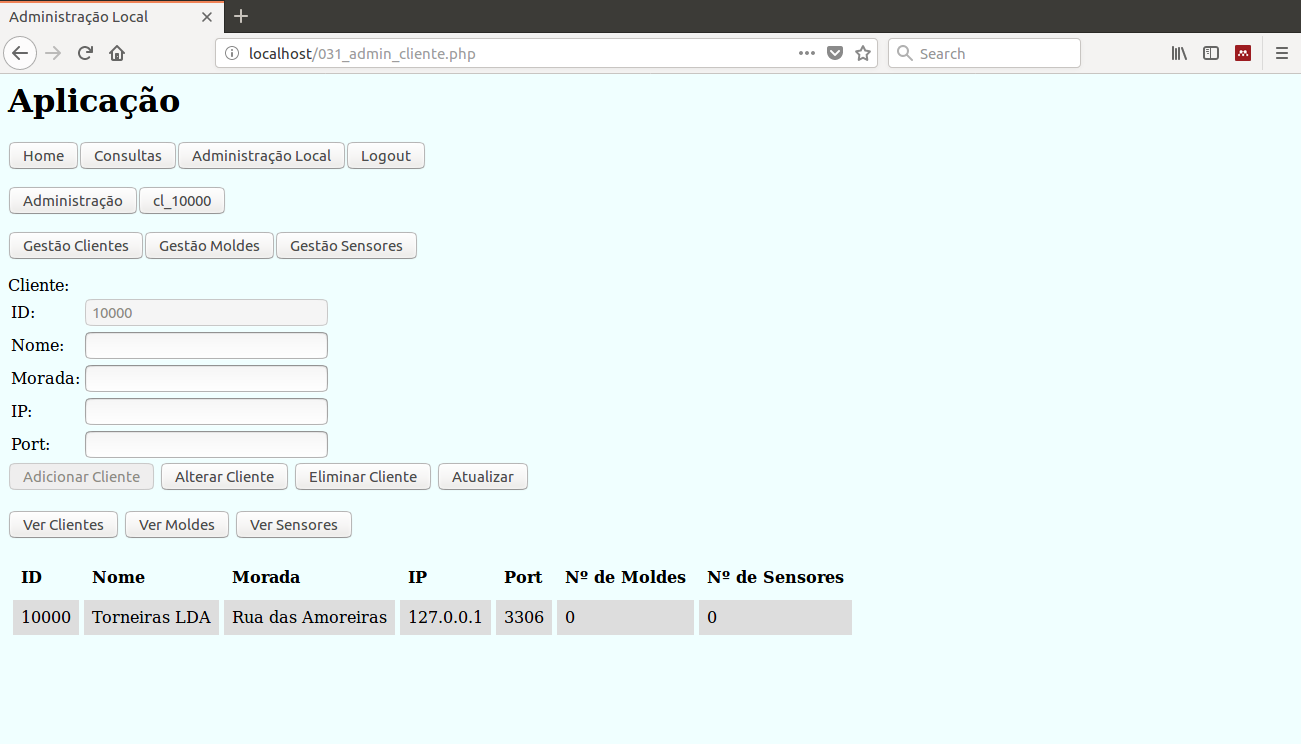
\includegraphics[width=0.9\textwidth]{futuro01} % Include the image placeholder.png
		\caption{Área de Criar Local com criação via \textit{root} em vez de gerar \textit{queries} para o utilizador inserir manualmente no \textit{MySQL}}
		\label{fig:conclusoes1}
	\end{center}
\end{figure}
Além disto é necessário realizar uma revisão de segurança à aplicação. Por exemplo, o botão Atualizar na área Gestão de Clientes que reinicia o programa de transferência de valores através de comandos no terminal. Se as permissões garantidas ao servidor \textit{Apache} não forem bem definidas, pode constituir uma quebra de segurança. Um programador com intenções maliciosas pode acessar o sistema pela aplicação e realizar comandos no terminal de forma a comprometer o sistema. Para isto não acontecer é necessário garantir que o servidor \textit{Apache} só tem permissões sobre o programa de transferência ou então definir um sistema de notificações entre a aplicação e o programa em \textit{C}.\\
Apesar de serem necessários alguns ajustes de forma a melhorar performance, a solução proposta da infraestrutura e aplicação é completamente funcional e pode ser já implementada numa fase experimental.

\section{Trabalhos Futuros}
Quanto à infraestrutura dos dados não foi definido como os sensores dos moldes serão ligados ao servidor local. No desenvolvimento deste projeto assumiu-se que todos os moldes estão ligados diretamente ao sistema local. Se esta proposta não se demonstrar viável é possível, em vez de se ter um servidor local por cliente, ter um servidor local por molde. Esta adaptação irá criar uma maior quantidade de bases de dados locais mas, isto não é problemático, se o modelo de dados e o programa de transferência forem adaptados para o efeito.\\
Quanto à aplicação, sugere-se que após uma apresentação inicial desta à empresa promotora, seja iniciado um processo iterativo de desenvolvimento para escolher e desenvolver novas funcionalidades que possam ser úteis e que não tenham sido abrangidas neste projeto, como por exemplo, a criação de utilizadores baseado no ID de trabalhador demonstrado na \autoref{fig:conclusoes2}. Culminando numa estilização da aplicação para que esta tenha um aspeto mais amigável ao utilizador.
\begin{figure}[H]
	\begin{center}
		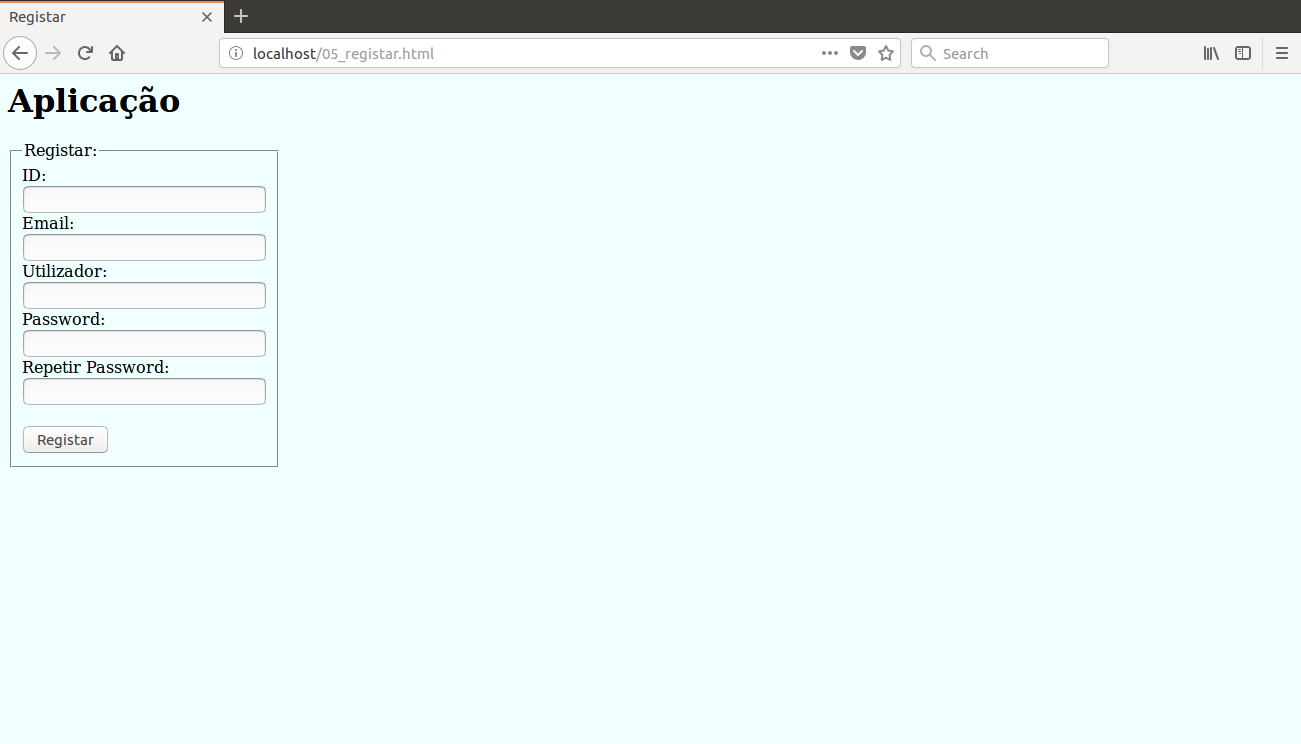
\includegraphics[width=0.9\textwidth]{futuro02} % Include the image placeholder.png
		\caption{Exemplo de área de Registar para criar utilizadores com base no ID de trabalhador e email}
		\label{fig:conclusoes2}
	\end{center}
\end{figure}
\vspace{-.82cm}
Além destas alterações sugere-se a criação de um sistema de notificações e monitorização automático dos moldes. É impossível para um utilizador analisar manualmente milhões de registos de um molde e concluir se este está a funcionar corretamente. Para este efeito criar um programa capaz de correr algoritmos que analisem o comportamento dos moldes. Este programa pode ser desenvolvido em \textit{softwares} mais sofisticados, como por exemplo \textit{MATLAB}, desde que estes tenham protocolos de comunicação com \textit{MySQL}.\looseness=-1\\
A gestão dos \textit{backups} descrita na \autoref{subchap:backups} onde se separa os registos dos moldes em vez de se realizar um \textit{backup} geral foi realizada com este sistema de notificações em mente. Se for necessário, para efeitos de cálculo, que o programa carregue os registos de um molde armazenados em \textit{backups}, este só necessita de carregar a informação do molde que está a ser analisado em vez de ter de carregar a informação de todos os moldes. Este programa deverá correr automaticamente no sistema de forma permanente ou com um temporizador e, no caso de ser necessário, notificar o utilizador via aplicação ou via email.

%
% The bibliography
%
\cleardoublepage
\bibliographystyle{unsrt}
\bibliography{bib/own/molde.bib,bib/own/base_dados.bib,bib/own/software.bib}

%%\sloppy
%%\printbibliography[prenote=myprenote,title=References]
%\iffalse
%  % Use this is the final version
%  %  unsrt produces numbered entries, sorted by order of citation
%  %  plain produces numbered entries, sorted alphabetically
%  %  other styles are possible (I recommend the harvard package)
%  \bibliographystyle{unsrt}
%  %\bibliographystyle{plain}
%  \bibliography{molde}% replace by the name of name of your .bib file
%\else
%  % An example (the contents of the .bbl file)
%  \begin{thebibliography}{10}
%
%  \bibitem{Eliahou-1-1993-CLBNCL}
%  Shalom Eliahou.
%  \newblock The $3x+1$ problem: New lower bounds on nontrivial cycle lengths.
%  \newblock {\em Discrete Mathematics}, 118(1--3):45--56, 1993.
%
%  \bibitem{Garner-1981-1-OCA}
%  Lynn~E. Garner.
%  \newblock On the collatz $3n+1$ algorithm.
%  \newblock {\em Proceedings of the American Mathematical Society}, 82(1):19--22,
%    May 1981.
%  \end{thebibliography}
%\fi
\cleardoublepage

\end{document}
